\documentclass{literature}

\title{Star Formation History}
\subtitle{First year report \& literature review}
\author{Owen J. Turner}
\authoremail{turner@roe.ac.uk}
\supervisor{Dr. Michele Cirasuolo}
\supervisoremail{ciras@roe.ac.uk}
\slugheader{First year report \& literature review}
\slugauthor{Owen J. Turner}
\logo{/Users/owenturner/Documents/PhD/KMOS/Latex/Literature_Review/UoEcrest.pdf}
\graphicspath{{Users/}{owenturner/}{Documents/}{PhD/}{KMOS/}{Latex/}{Literature_Review/}{Figures/}}
\abstract{}
\setcounter{secnumdepth}{4}


\begin{document}

\background
\label{background}



%%%%%%%%%%%%%%%%%%%%%%%%%%%%%%%%%%%%%%%%%%%%%%%%%%%%%%%%%%%%%%%%%%%%%%%%%%%%%%%%%%%%%%%%%%%%%%%%%%%%%%%%%%%%%%%%%%%%%%


\section{Meetings with Michele}\label{meetings}
\subsection{21-10-14}\label{meeting_1}
Mainly we discussed Stellar population synthesis models, going through the details of the grid of stellar evolutionary tracks. There are a series of steps: 
\begin{itemize}
\item We know the evolutionary path on the HR diagram with stellar evolution models. Therefore for each mass of star we know how long it will live for 
\item Draw the lightcurve for each individual star to know how much it is emitting as a function of time 
\item Convolve this with the assumed IMF of the galaxy, given as either the Kroupa form \citep{Kroupa1993}, or the Chabrier form \citep{Chabrier2003}, which then weights these lightcurves by the total number of object of given mass. 
\item This produces a synthesised lightcurve at a particular snapshot in time for the entire population of stars 
\item Can repeat this procedure at any time to get a set of models of different ages 
\item Things become more complicated when the star formation history and supernovae are included, as essentially the models are functions not just of the IMF and age, but also of the metallicity and star formation history. Supernovae enrich the ISM gas with metals with each generation of star formation, and blow some gas out of the galaxy completely. 
\item Convert to a plot of flux versus wavelength with stellar atmosphere models, which describe the variation form blackbody emission for the stars   
\end{itemize}
That's essentially the picture - there is inherrent uncertainty in the resultant global emission due to the modelling process and much work went on between the Kennicutt review and the update in refining these SPS models. $\chi ^{2}$ minimisation procedures used to select which model has the best fitting parameters to the data observed across as many wavebands as possible (with dust added manually afterwards). Star formation rate inferred from the best fitting model. \\
We also discussed the four major SFR diagnostic methods, these being UV, FIR, Radio and emission lines. To get the relations given by Kennicutt between the UV, FIR flux and SFR, restrict the models to a particular part of the spectrum and find out how much star formation you would require to produce that amount of flux. \\
In sum, we model how much emission is produced across the spectrum, the SED, for a galaxy. These models depend on age, metallicity, redshift, star formation history and dust. We observe the galaxy in as many wavebands as possible and then fit the model to the data with the parameters allowed to vary. If we have enough data points we can break the degeneracy between age and redshift and determine in a $\chi ^{2}$ minimisation and then marginalisation procedure what the best fitting parameters are. Hence we know about the best fitting parameters for that galaxy, one of which is the SFR. Need to think about this more in terms of the ultimate goal being model fitting - the data collection is a means to this end. Next thing to move onto is reading about how the metallicity can be meaured for a galaxy. 
\subsection{28-10-14: Cosmology Calculator Task}\label{meeting_2}
Met to discuss the cosmological distance calculator task. Set the task of computing the luminosity distance, angular diameter distance, volume and age of the universe at a given redshift, given a particular cosmology and hubble parameter. This is done via numerical integration of the equation which defines the comoving distance: 

\begin{equation}
D_{c} = D_{H} \int ^{z} _{0}\frac{dz\prime}{E(z\prime)} 
\end{equation}

Where $E(z) = \sqrt{\Omega _{m}(1 + z)^{3} + \Omega _{k}(1 + z)^{2} + \Omega _{\Lambda}}$. This will be done using trapezoidal methods, the simpson rule, Romberg quadrature and gaussian quadrature. The luminosity distance is absolutely crucial in observational astronomy, as this is the distance which is used when converting between flux and intrinsic luminosity of the source.

\begin{figure}[!htp]
\centering
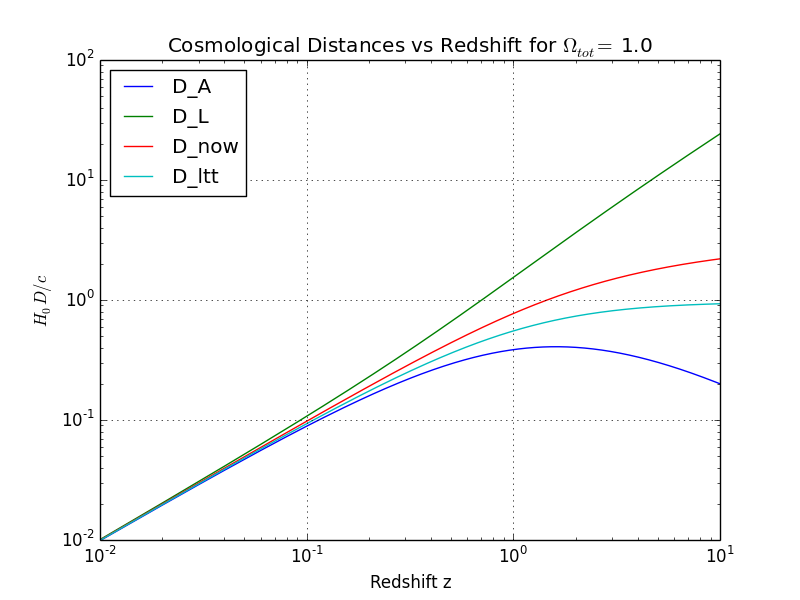
\includegraphics[width=0.8\textwidth]{cosmo_dist.png}
\caption{\footnotesize{\emph{Plot of the different cosmological distance measures against redshift}}}
\label{fig:cosmo_dist}
\end{figure}

\subsection{4-11-14: Spectra Task}\label{Meeting_3}
Following the cosmological calculator, emission line fluxes can now be turned into the physical properties of galaxies using the luminosity distance. The task is now to go to the SDSS, take a galactic spectra and play around with fitting polynomials to the continuum, gaussian peaks to the emission lines to get the fluxes, the equivalent widths, BPT diagram, redshift etc. The easy step is then coding the computation of the physical quantities after extracting these values. \\\\
\noindent
Michele suggests that coding in a modular way is the best way to do this. e.g. have a module which loads in the fits file in the first place given a list of ID's, then a module which computes the redshift from the plotted spectra, then a module which locates the emission line peaks given the redshift of the galaxy, then a module which computes the physical quantities once the rest has been done. Got an email from Michele on this date listing the SDSS references, data access files and papers to consult whilst attempting to do this. The stress here is definitely on taking the spectra and playing around with it. Try different things, look at how the continuum could be fit by masking out the emission lines, or by using a polynomial of high order. Probably the best thing to do would be to smooth the spectrum using the moving average function defined already, subtract this from the data, fit the continuum, divide the original spectrum by the continuum spectrum and then proceed to do some science from that. \\\\
Also asked Michele some questions about the process of determining metallicity in general. Line fluxes bear some relation to atomic abundance. These relations need to be calibrated theoretically by using codes like cloudy, or empirically by looking in the local universe at the electron temperature and density, which are better resolved there and then extending this to higher redshifts. The reason for expressing the abundance in terms of log(OH) is just as a normalisation factor. 
\subsection{13-11-14: Meeting after spectra task}\label{Meeting_4}
Discussing my initial attempt at the spectra task and taking a look at some of the results. So I think I did an okay job but the continuum fitting isn't quite right, which in turn is affecting the way that the gaussians are being fitted to the emission lines. Instead of blindly fitting a polynomial I should be masking off the emission lines in some way. Michele suggested the local continuum method, whereby in the vicinity of emission lines I estimate the local continuum and subtract this at each stage before fitting the line profile. Also since the gaussian models seem to underestimate the peaks of the emission lines, Michele suggested using a two gaussian fit, to account for broader features at the base of the line profile which are causing the peak of the gaussian to fall too early. Also binning up the continuum to get a better signal to noise from the continuum subtracted data. \\
How to estimate the error on the line fluxes? Extracting the errors on the individual flux points, which comprise the emission line profile. Then for each of these points generate gaussian random variables with mean value of the original datapoint and sigma of the point error. For all of the points which make up the peak, draw this random variable and then fit a gaussian to this and compute the flux, store this in a vector. Do this 100 times to get a distribution of fluxes, the resulting standard deviation of this gaussian is the overall error on the flux. Monte Carlo error estimation. \\ 
Finally Michele suggested that I be given some spectral templates to cross-correlate with these SDSS spectra in order to determine the redshift. Two different techniques for doing this - one applicable in the high signal to noise regime, this being the simple cross correlation function (shift and compute probability, then plot probability against redshift) and another for the low Signal to noise limit where individual probability spikes won't be visible in the cross correlation function. This second method minimises $\chi ^{2}$ but requires an additional fudge factor to accurately explore the two dimensional $\chi ^{2}$ surface. \\ 
Tasks are: 

\begin{itemize}
	\item better explore the continuum with the techniques suggested by Michele 
	\item Continue to read the Kewley and Dopita theory paper 
	\item fit double gaussian line profiles 
	\item continue to play with the data and figure how to mask emission lines etc 
	\item cross correlation functions from different galaxy spectral templates to determine the redshift
	\item Monte Carlo error estimation for the line fluxes
\end{itemize}

An initial plot of the different galaxy templates looks like this: 

\begin{figure}[!htp]
\centering
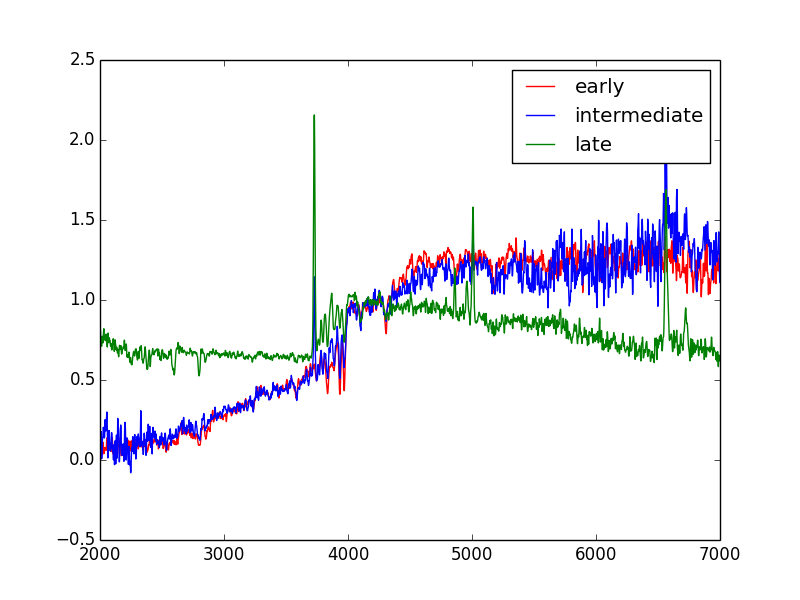
\includegraphics[width=0.8\textwidth]{spectral_templates.png}
\caption{\footnotesize{\emph{Plot of the spectral flux templates on the same axes}}}
\label{templates}
\end{figure}

Also was looking at Fergus poster in the corridor and a few points stood out. The physical process driving the mass metallicity relation is that galaxies require pristine gas in order to form stars, more massive galaxies drag in more of this from the IGM due to their increased gravitational potential and also hold onto more of their enriched gas for the same reasoning. So it would be expected that the most massive galaxies are also the most metal enriched. \\ 
Also it would appear that Fergus is fitting all of his emission lines simultaneously using a composite model, rather than fitting the lines individually. Should maybe attempt to do this again because this seems to be the way it is done in all of the papers. \\

\subsection{3-12-14: Continuing with spectrum fitting and python}
I decided to collate everything into a class after the visit from Claude. Much better organisational structure and can be easily imported into any program afterwards. Made class objects for both the observed and template spectra - called spectrumFit and templateSpec. Also have the Monte-Carlo flux error, the equivalent width and the equivalent width error working. All of the methods are stored within the spectrumFit class and can be found either locally or on github.  

\begin{figure}[!htp]
\centering
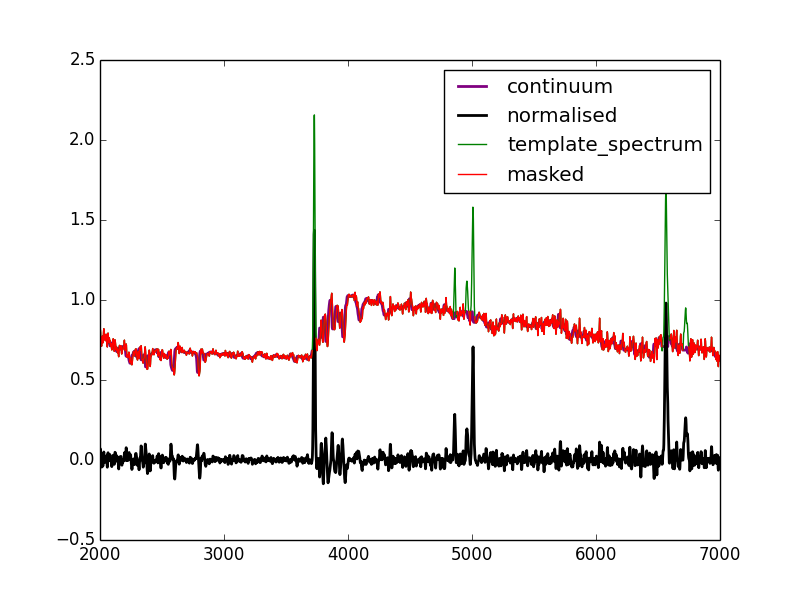
\includegraphics[width=0.8\textwidth]{template_spectrum.png}
\caption{\footnotesize{\emph{Plot of the normalised late type galaxy spectrum}}}
\label{fig:norm_temp}
\end{figure}

\begin{figure}[!htp]
\centering
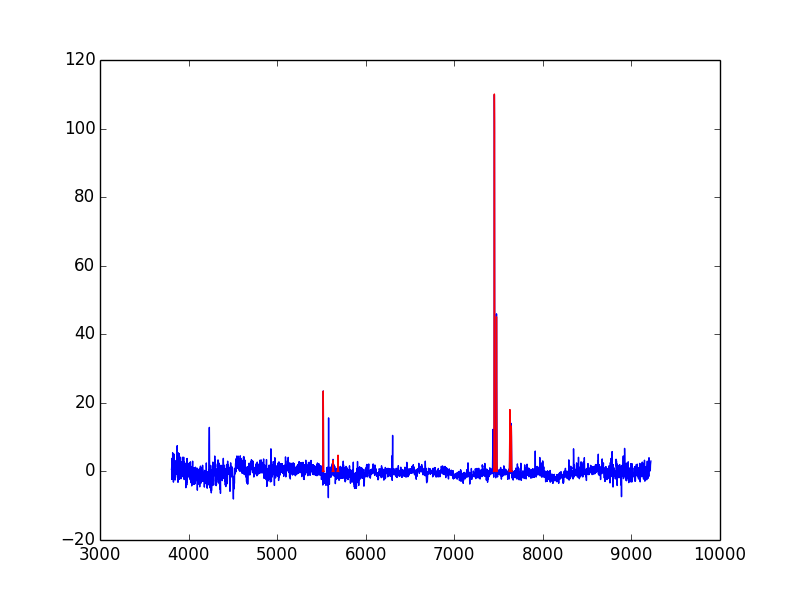
\includegraphics[width=0.8\textwidth]{fitted_spectrum.png}
\caption{\footnotesize{\emph{Plot of one of the fitted SDSS galaxy spectra}}}
\label{fig:fit_spec}
\end{figure}

\subsection{4-12-14: Introduction to KMOS}
Met with Michele and discussed an alternative recipe for computing the redshift from a template spectrum, by using a redshift grid and interpolation at each stage, instead of a single wavelength transformation to one grid. Will try this out. Also started discussing the main science aims of Michele's next observing run, the potential science goals of my PhD and the beginning stages of understanding the KMOS analysis pipeline. Given a list of manuals to download and read and also the link to the analysis pipeline so that I can begin installing the software and using test data to see if I can get this to work. \\
KMOS produces 3D cubes, where two of the directions are the physical x and y information on the sky, and the third axis is the wavelength information after the light has been dispersed by the spectrograph. KMOS has 24 arms and so the first step is to choose the targets. Once these have been confirmed, the instrument slices the light from each of the arms into cubes of 14x14 pixels. These are fed into the disperses and for each of these individual pixels a spectrum is recorded. The instrument has 3 detectors, each of which picks up 8 objects and so the final fits file spat out by the telescope has 3 images, each of which contains 8 14x14 spectra. \\ 
Michele's work at the moment is focussing in on redshift 3-5 galaxies, with known redshift values, which we want to study the spatial gradients of metallicity, SFR and velocity within. Knowing how these values shift radially within a galaxy gives access to information about how the products of star formation are distributed within a galaxy. A lot of information to digest at once, as Michele will be in Chile for the following but we discussed the major stages of every analysis pipeline; bad pixel and dark current subtraction, flatfielding, wavelength calibration, flux calibration; and also the KMOS specific stages, reconstruction of the 3D KMOS cube and then stacking of the observations which are taken in OSO-OSO.  \\
Finally got the redshift template method working using the new approach suggested by Michele, the only problem is that it runs quite slowly compared to the other way. If there was a way to get the other method to work this would be much prefered, but the redshift output of the new method matches closely to the SDSS line redshift solutions. SDSS appear to have a redshift solution for each individual spectral line - could proably figure out how to do this if more time was spent. But now will focus on the KMOS analysis. 

\begin{figure}[!htp]
\centering
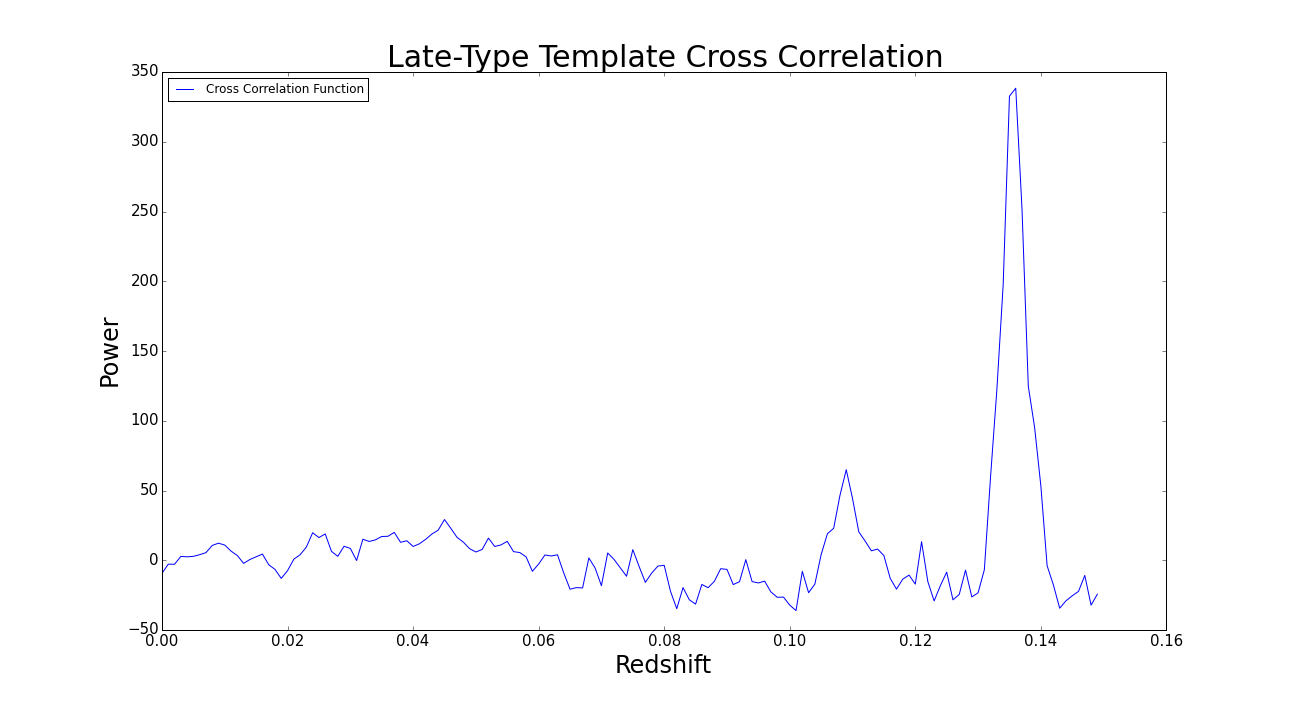
\includegraphics[width=0.8\textwidth]{Cross_corr.png}
\caption{\footnotesize{\emph{Plot of one of the working CCF}}}
\label{fig:cross_cor}
\end{figure}

Received some test KMOS data from Michele and have installed the pipeline properly (hopefully) so will try running through the whole pipeline from the tutorial book. Need to use the easySPARK.sh files, with the sof extension at first to create the list of files and check that the correct list has been created. Need to have the same dark exposure time and exposure time on the source, so need to use the dark frames with the correct exposure time in the preparation files. Use dfits and fitsort first to search through the properties of the files to know which are the correct ones to use in the pipeline. Spits out files at different stages before eventually reconstructing the data cube. Needs to be 2D to do all of the standard data analysis stuff.




\section{Journal}
\subsection{8-12-14: Introduction to KMOS}
Data reduction session with the KMOS data from Michele. I'll try to keep a note of progress here, the things I'm trying and that commands I'm using to do this and questions for Michele at the end of this. First is the correct use of the dfits command: \\

dfits `filename.fits' `pipe' fitsort exptime \\ 

For example would take the file and list the exposure time on the source. Useful when dealing with dark frames, as the dark frame exposure must be the same as the source exposure to be able to accurately subtract the dark current. Will give more examples in the literature book as I go along. \\ 
The standard star spectral irradiance calibrations are derived from the NIR magnitudes of stars reported by Cohen \citep{Cohen2003}. This is from the 2MASS survey \citep{Skrutskie_2006}. The Telluric spectrum is trickier, this was perhaps attempted automatically during the recipe. Otherwise there is an excellent option for producing Telluric spectra described by Vacca \citep{Vacca2003}. \\ 
\textbf{Science Reduction} \\ 
Everything has been done as described apart from the illumination correction, which I couldn't get to work properly. The Telluric correction did work, it is these two files which are not manadatory for the science reduction stage. \\ 
Went through all the stages and got some data cubes, but no idea how these should look. Not sure whether this is a problem with my qfitsview as the statistics for the cubes seem pretty solid. 


\subsection{10-12-14: Continuing with KMOS reading}
Managed to install Anaconda with python 2.7.8. Briefly was using python 3.4, which is the first ever backwards incompatible python release - it was total rubbish and none of my programs worked with it. Was easy to revert to the other version of python and got everything working again yesterday after a stressful period of mucking around. Now also have the qtconsole ipython viewer with inline matplotlib plotting, will be handy when trying to visualise a certain piece of work. Get syntax highlighting and can run scripts from within there. \\ 
Reading the KMOS introduction slides - commentary on this primary in the Literature book. Not very useful, need to understand the instrument better first before attempting the reconstruction again. Main problem is qith qfits not working properly - I think that I have a reconstructed data cube but I'm not sure how to view this. The end results in the slide look really cool, want to be able to get to this stage, but requires a lot of customisation of the pipeline analysis. \\ 
\textbf{VLT MANUAL} \\ 
The key feature of KMOS is its ability to perform Integral Field Spectroscopy in the near-infrared bands for 24 targets simultaneously. The instrument design employs 24 configurable arms that position pickoff mirrors at user- specified locations in the Nasmyth focal plane. The sub-fields thus selected are then fed to 24 image slicer integral-field units (IFUs) that partition each sub-field into 14 identical slices, with 14 spatial pixels along each slice. EXPLANATION OF THIS SECTION. How does the image slicer work and how can I visualise the 14 spatial pixels along each of the 14 identical slices? Light from the IFUs is then dispersed by three cryogenic grating spectrometers which generate 14x14 spectra with $\sim$1000 Nyquist-sampled spectral resolution elements for each of the 24 independent sub-fields. The patrol field of the pickoffs is 7.2 arcmin in diameter, which is the diameter of the unvignetted field at the VLT Nasmyth focus, thus minimising the thermal background in the K- band. Each IFU has a square field of view of 2.8 x 2.8 arcsec; anamorphic magnification in the IFU foreoptics ensures uniform spatial sampling of 0.2 x 0.2 arcsec whilst maintaining Nyquist sampling (~2 pixel) of the spectral resolution element at the detector. Crucially the pickoff arms can patrol a very wide field of 7.6arcmin, and then the field of the IFU is square and 2.8x2.8 arcsec, giving each pixel a spatial sampling of 0.2 arcsec. Below is a visual example of integral field spectroscopy. Really good descriptions of each of the concepts in the VLT manual written by Michele. Should return here when trying to create the presentation and when writing any of this up. 

\begin{figure}[!htp]
\centering
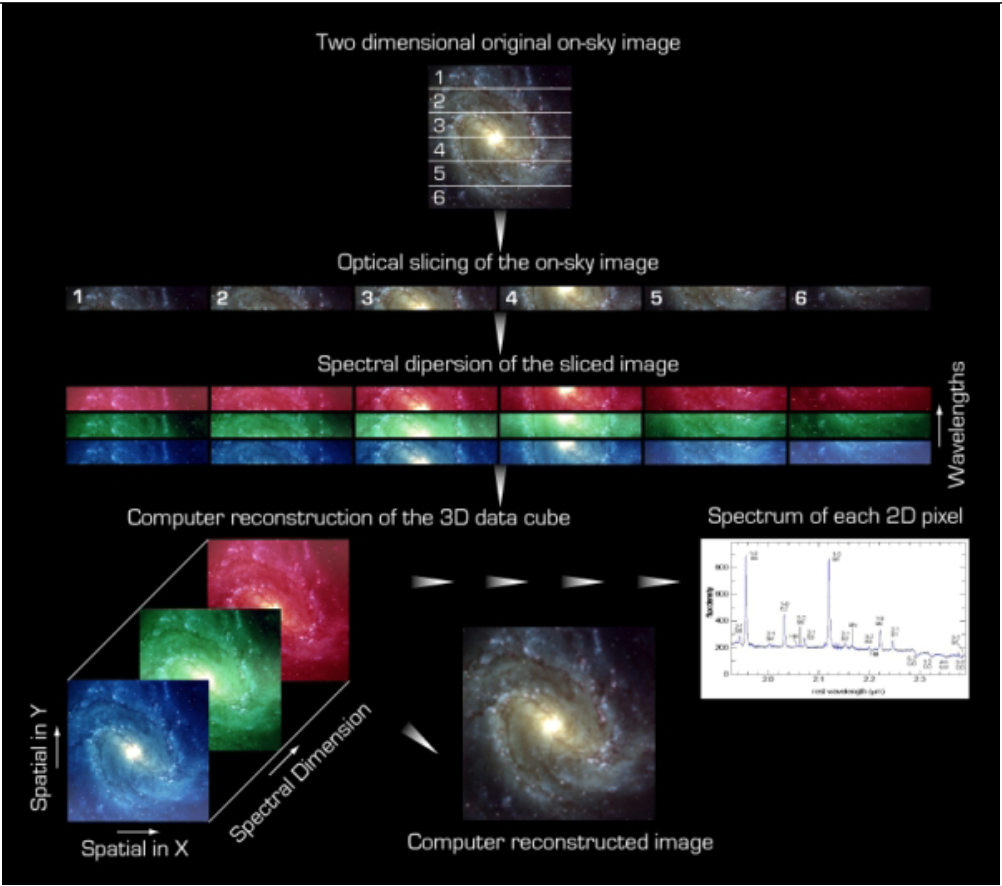
\includegraphics[width=0.6\textwidth]{kmos_disperse.png}
\caption{\footnotesize{\emph{Example of Integral Field Unit Spectroscopy. A 2-dimensional image will first be sliced, the slices then dispersed on a common slit and finally a 3D data cube is reconstructed from the obtained spectra. In KMOS the image is sliced in 14 elements instead of 6 as in this figure}}}
\label{fig:kmos_disperse}
\end{figure}

\begin{figure}[!htp]
\centering
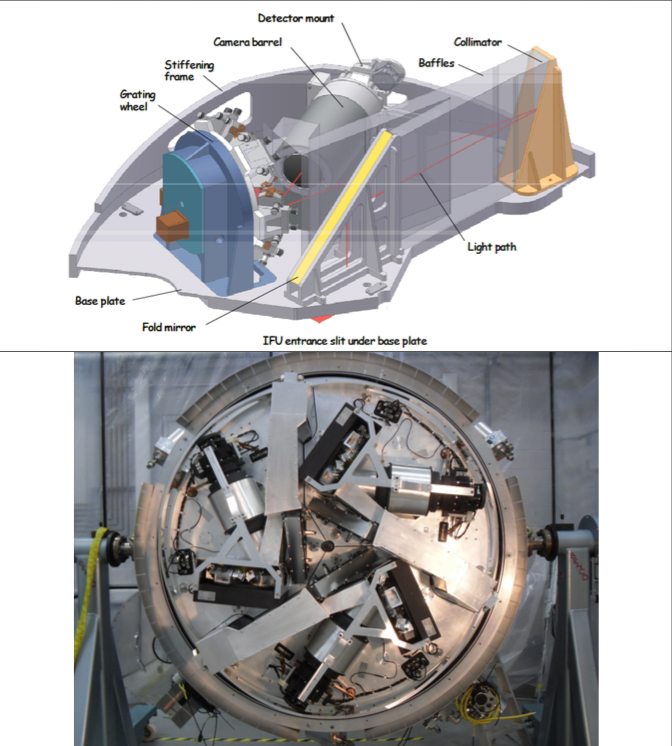
\includegraphics[width=0.6\textwidth]{kmos_speectrographs.png}
\caption{\footnotesize{\emph{Perspective view of the mounted KMOS spectrographs inside the cryostat}}}
\label{fig:kmos_spectrographs}
\end{figure}


\textbf{Questions}
\begin{itemize}
\item Environment variables? Is it wise to start a seperate data reduction `session' with different folder names each time I'm working on this? 
\item The different wavebands. What is contained in the fits files I'm looking at? Are these combined images from all the different NIR bands? 
\item Why are the exposure times on the standard stars, the objects we are using to calibrate flux, so much less than on the target objects? Shouldn't something being used to calibrate flux be collecting photons over an equivalent base timescale? 
\item Matching arcs and flatfields - getting the same rotation angles for these. Get the best results by using them in `sets' 
\item The importance of the illumination correction when processing science data
\item How to ensure the consistency of the flat and arc calibration products 
\item How important is it to know what the recipes are doing?
\item In step 4.3, the wavelength calibration using the arc frames, one of the end products is lcal.fits, which is a frame containing the wavelength values of every pixel on the detector. How does this work? Is the light in every pixel dispersed? No the target is selected by one of the IFUs, each of which has this 14x14 array of pixels and then this light is fed into the disperser... Does this individually disperse the light in each of the 196 pixels? 
\item what am I looking at in det-img-wave.fits? 
\item Due to the differential flexure of the instrument between the flatfield and the sky exposures. What is differential flexure? 
\item How do we use the illumination correction frame after it has been created? 	
\item Am I meant to be using the standard stars inside the Galaxy folder, or the standard stars which are in the calibration folder? These both seem similar. 
\item What should I be seeing when I open the standard star cube in qfits? At the moment getting nothing both when trying to open this and when trying to open standard fits files (which aren't cubes)
\item What is the importance of the Telluric spectrum? Is it created and then used immediately? Because there are no output files described in that section of the data reduction. No Telluric was produced.
\item I'm missing something - the difference between integral field and multiple object spectroscopy. Is is that each IFU selects an extended target, the image is sliced, fed through the lenslet array and then dispersed and the multiple object part is that this is happening simultaneously for lots of different objects in the field of view? 
\item A datacube has three axes - the x and y coordinates of the object on the sky and the wavelength axis. How then do we get the spectra, which is the distribution of energies in this space?? Usually when we see a spectrum is it just energy against wavelength, so how do the x and y axes fit into this? 
\item Page 7 of the KMOS tutorial slides, the detector raw images. What am I actually looking at there? Can see the single spatial of wavelength dimensions, what is being dispersed? 
\item Full example of what I'm looking at in one of the OBS.fits files
\item qfits won't even open regular fits files let alone reconstructed data cubes
\item Image slicer question in the above section
\item What is a 14x14 spectrum? 
\item Surely each of the 24 pickoff arms are focussing on seperate fields of view. How then can 8 of these be combined to give a single image on a detector? E.g. the continuous line across the detector image when iluminated with the Neon light 
\item How to extract a 1D spectrum from a 2D spectrum e.g. steidel
\end{itemize} 

\textbf{Observing with KMOS} \\

The figure below shows an image from KARMA, the observation preparation tool for KMOS. Special algorithms for maximising observation targets, given a particular field of view, which minimise the chance of arm collisions and confusion.

\begin{figure}[!htp]
\centering
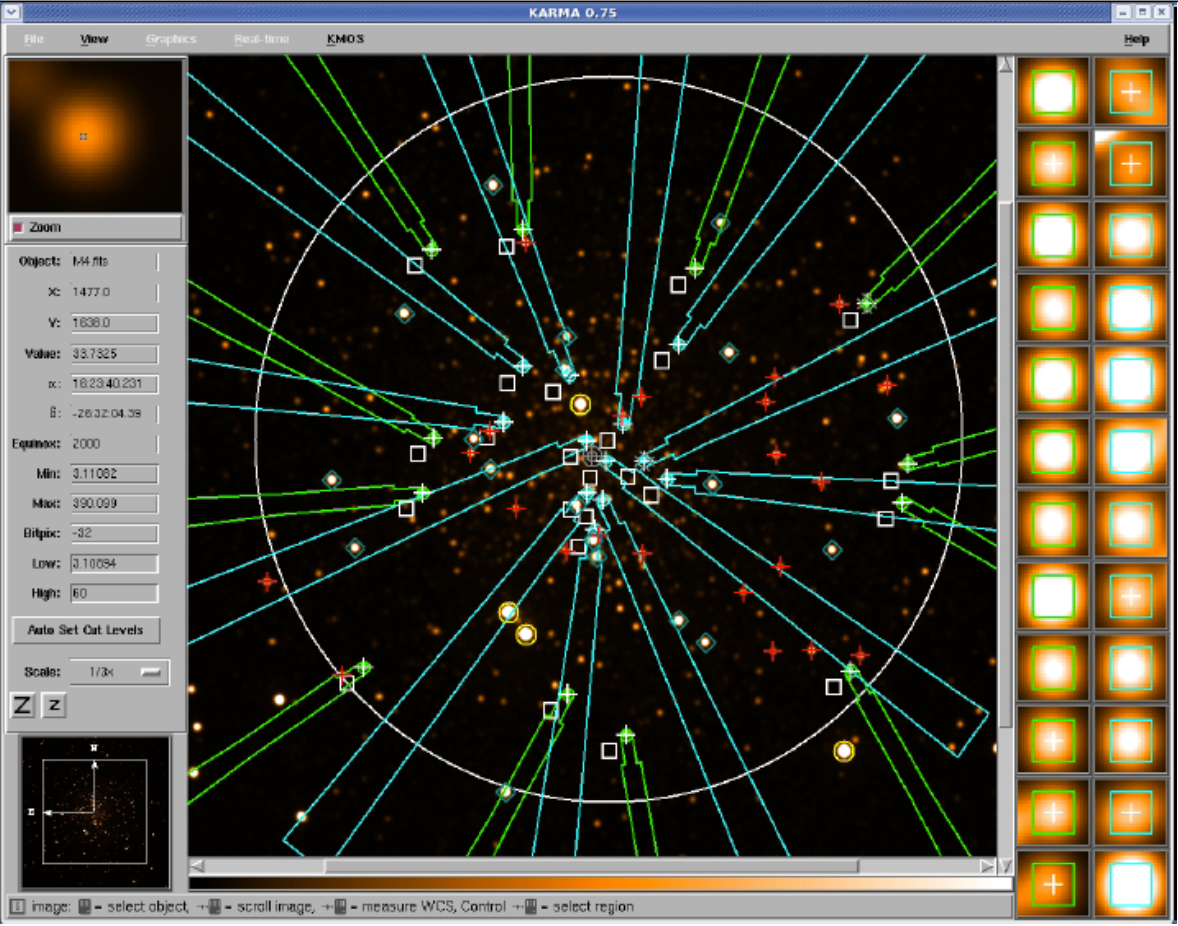
\includegraphics[width=0.6\textwidth]{kmos_karma.png}
\caption{\footnotesize{\emph{View of observation preparation using KARMA}}}
\label{fig:kmos_karma}
\end{figure} 



\textbf{Questions}
\begin{itemize}
	\item KMOS observations are all coded using templates - what does this mean? Two or more templates make an observing sequence
\end{itemize}


%%%%%%%%%%%%%%%%%%%%%%%%%%%%%%%%%%%%%%%%%%%%%%%%%%%%%%%%%%%%%%%%%%%%%%%%%%%%%%%%%%%%%%%%%%%%%%%%%%%%%%%%%%%%%%%%%%%%%

\section{Kennicutt 98: Star Formation in Galaxies along the Hubble sequence}

\subsection{Introduction}
Properties which are affecting the large scale star formation rate within galaxies: 
\begin{itemize}
\item Morphological type 
\item Gas content 
\item bar structure 
\item dynamical environment
\end{itemize}

The first precise diagnostic techniques for measuring the SFRs of galaxies came in the 1970's and 1980's and included integrated emission line fluxes (Cohen 1976, Kennicutt 1983a), near ultraviolet continuum fluxes and IR continuum fluxes. More techniques developed as technology advanced. Interest in the field developed hugely over the following decade, due to two major revelations. The first was the discovery of a population of ultraluminous IR starburst galaxies (ULIRGs) by the Infrared Astronomical Satellite (IRAS) in the mid 1980's, an ubiquitous and extreme phenomenon. The second is the discovery of SFGs at high redshift, $z \sim 3$, allowing for the locally calibrated SFR diagnostics to be applied to distant galaxies and to directly trace the evolution of the SFR density and the Hubble sequence as a function of cosmic lookback time. Galaxies exhibit a huge dynamic range in SFRs, over six orders of magnitude even when normalised per unit area and galaxy mass.

\subsection{Diagnostic Methods}
Since individual young stars are unresolved in all but the closest galaxies, even when using HST, most of the information surrounding the SFR comes from integrated light measurements in the UV and FIR and from nebular recombination lines. Synthesis modelling forms the basis of all the methods. 

\subsubsection{Synthesis Modelling}
Along the Hubble classification fork the spectra of galaxies change in several very noticeable ways. The blue continuum increases broadly, a gradual change in the composite stellar absorption spectrum from K-giant dominated to A star dominated and a drastic change in the strengths of nebular emission lines, particularly H$\alpha$. It is easy to show that the integrated light from stellar populations, although containing contributions from all stellar masses, is dominated from intermediate-mass main sequence stars. As a result the spectra and colors of galaxies fall on a relatively tight sequence, and the spectra of any particular object is dominated by the ratio of early to late-type stars. This makes it possible to use the observed colours to estimate the fraction of young stars and the mean star formation rate of recent times ($10^{8-9}$ years.) \\
The simplest application of this approach would be to assume a linear scaling between the SFR and the continuum emission integrated over a particular blue or ultraviolet bandpass. Although this is a good approximation for young star forming galaxies the assumption breaks down for older galaxies, where a considerable fraction of this continuum emission is emitted by the older stars in the population. The scaling between SFR and continuum luminosity is however a smooth function of the colour of the stellar population, and this can be calibrated using an evolutionary sythesis model. \\
A grid of stellar evolution tracks is used to derive the effective temperatures and bolometric luminosities for various stellar masses as a function of time. So the equations of stellar evolution are coded into a time, mass, age, metallicity, SFH grid, and the differential equations are numerically evaluated at each point so that the values of the effective temperature and bolometric luminosity can be read off for various stellar masses as a function of time. The individual stellar templates are then summed together and weighted by an IMF, Krupa or Chabrier, which has a tail off at the low mass end of the IMF, to synthesize the luminosities, colours, or spectra of single age populations as functions of age. These isochrones can then be added together in linear combination to synthesise the spectrum of colours of a galaxy with an arbitrary star formation history. The four free parameters usually used in these models are the star formation history, galaxy age, metal abundance and IMF. Widely used models of star forming galaxies include those of Bruzual and Charlot  (1993), Bertelli et al. (1994) and Fioc \& Rocca-Volmerange (1997). \\ 
The models generate the SFR per unit mass or per unit luminosity as a function of the colour of the galaxy. The broadband luminosity of the galaxy by itself is a poor tracer of the SFR, as the SFR is shown to vary by more than an order of magnitude over the relevant colour range in Figure 2 of this paper. We need more information about the emission of the galaxy as a function of wavelength. More photometric points, more details about age, metallicity, history. The SFRs generated in this way are relatively imprecise, prone to systematic errors arising from uncertain knowledge of the IMF, metal content, reddening and age. The method should be avoided in cases where these quantities are likely to change systematically across a population of galaxies. \\ 
\subsubsection{Ultraviolet Continuum}   
The above problems can be avoided by observing in a particular wavelength range that is free from the contamination of older stellar populations, and then assuming a linear relationship between the SFR and UV luminosity.The optimal wavelength range is 1250-2500 angstroms, longward of the Lyman alpha forest, but short enough to minimise the contamination from older stellar populations. This wavelength range is inaccessible from the earth for local galaxies (z   \textless 0.5), but can be observed in the redshifted spectra of galaxies with $z \sim 1-5$. The Keck telescope first observed the redshifted UV continuum in a large sample of galaxies with z \textgreater 3. The synthesis models are again used to calibrate the relationship between measured UV continuum and star formation rate. The most important thing coming out of this section is that it's important to apply an SFR calibration method that is appropriate to the population of interest. The real benefit of using the UV continuum method is that it relies upon measuring the photospheric emission of the young stellar population and it can be applied to star forming galaxies over a wide range of redshifts. As a result it is currently the most powerful probe of the cosmological evolution of the SFR \citep{Madau1996}. The chief drawbacks of this method are the sensitivity to extinction and the form of the IMF.
\subsubsection{Recombination Lines}
As is shown in Figure 1 of this paper, the most dramatic change in the integrated spectrum with galaxy type is a rapid increase in the strengths of the nebular emission lines, which effectively re-emit the integrated stellar luminosity of galaxies shortward of the Lyman limit and so are sensitive to the young massive stellar population. The only stars which produce this flux of ionising photons are the young and massive population, and so the strengths of the H$\alpha$ etc emission lines are directly proportional to the number of young stars and hence the star formation rate. The relationship between SFR and nebular line strength is calibrated using a stellar evolutionary synthesis model. The primary advantages of this method are the direct coupling between the nebular emission and massive star formation rate (the lower mass stellar population simply don't produce high enough energy photons) and the high sensitivity. As before, the limitations of this method are the uncertainties associated with extinction, the IMF and the assumption that all of the star formation is being traced by ionised gas. Estimates of the escape fraction are important when considering how to relate the nebular emission line strength to the SFR. The extinction of photons emitted from ionised gas clouds is the most important source of error, and the line of sight extinction can be estimated by comparing H$\alpha$ fluxes with IR recombination line fluxes. The ionising flux is produced almost exclusively by stars with M \textgreater 10 solar masses, and so the measured SFR is especially sensitive to the choice of IMF. However the H$\alpha$ line equivalent widths and galactic colours are sensitive to the slope of the IMF over a wide range of stellar masses and these can be used to constrain what that slope is. 
\subsubsection{Forbidden Lines}
Due to H-alpha being redshifted out of the optical window at z \textgreater 0.5, there is much interest in calibrating bluer emission lines as quantitative SFR tracers. However these are weaker and more susceptible to stellar absorption. The strongest emission feature in the blue is the OII forbidden line doublet. Forbidden lines are not directly coupled to the ionising luminosity, however OII is well behaved enough that it can be empirically calibrated using H$\alpha$ as a quantitative SFR tracer. The main advantage of using this emission line is to examine the SFR and hence SFH up to higher redshifts and lookback times. Especially useful when used to look at high redshift galaxies, and as a consistency check of SFRs derived in other manners.
\subsubsection{Far-Infrared Continuum}
A significant fraction of the bolometric luminosity of a galaxy is absorbed by interstellar dust and re-emitted in the thermal IR, at wavelengths of roughly 10-300$\mu m$. Since the dust is preferrentially absorbing in the UV, in principle the FIR emission can be a sensitive tracer of the young stellar population and the SFR. The efficacy of the FIR emission as a tracer of SFR, depends upon the contribution of young stars to heating of dust, and on the optical depth of dust in star forming regions. The simplest physical situation where this could apply would be a galaxy in which the UV-optical continuum emission is dominated by the young stellar population, and the dust opacity is high everywhere. Then the strength of the FIR emission is just directly proportional to the SFR, with the measurement being calorimetric. The real physical situation is more complex than this in the disks of normal galaxies. There are two components to the dust spectrum: The First a warm component, coming from the heating of the young stellar population with $\lambda _{peak} = 60\mu m$ and a cooler component ($\lambda _{peak} > 100\mu m$) arising in more diffuse dust clouds heated by the ISM radiation field. In blue galaxies both components can be the result of the young stellar population, but in red galaxies there are far less young stars and dust heating from the visible spectra of old stars may become very important. As a result of these two components, directly relating the FIR emission to SFR is a controversial topic and the calibration is not straight forward.
\subsection{Disk Star Formation}




%%%%%%%%%%%%%%%%%%%%%%%%%%%%%%%%%%%%%%%%%%%%%%%%%%%%%%%%%%%%%%%%%%%%%%%%%%%%%%%%%%%%%%%%%%%%%%%%%%%%%%%%%%%%%%%%%%%%%%



\section{Kennicutt 2012: Star Formation in the Milky Way and Other Galaxies}
\subsection{Star Formation Rate Diagnostics: The Impact of Multiwavelength Observations}
This section is describing the improvements in calibration and validation of the diagnostic methods for determining SFRs in galaxies. Updated synthesis modelling, IMFs, modelling of dust etc have all contributed towards reducing uncertainties, by up to an order of magnitude in several cases.
\subsubsection{Star Counting and analysis of the colour magnitude diagram}
Having the resolution to count individual stars within galaxies and use the formula given on page 545 to find the SFR. 
\subsubsection{UV Continuum Measurements: The Impact of GALEX}
For a conventional IMF, the peak contribution to the UV flux shortwards of the Lyman-continuum is from stars with several solar masses. Hence measurements of this continuum should in theory directly trace stars formed over the past 10-200Myr. GALEX revolutionised this area, imaging two-thirds of the sky in the FUV(155nm) and the NUV(230nm) channels \citep{Martin2005}. This was the first space based UV mission and so provided integrated UV fluxes and hence SFR estimates for hundreds of thousands of galaxies. 
\subsubsection{Emission Line Tracers}
For a conventional IMF these lines trace stars with masses greater than 15 solar, with peak contribution from stars in the mass range 30-40 solar. As such, the lines provide a nearly instantaneous measure of the SFR, tracing stars with lifetimes of 3-10Myr. \\ 
Why isn't Lyman-a used instead of H-a? The strength of the former is 8.7 times that of the latter in Case B recombination, making it an attractive tracer in pricinple, but in realistic ISM environments the line is subject to strong quenching from the combination of resonant trapping and the eventual absorption by dust, usually quantified in terms of a Lyman-a escape fraction. 
\subsection{Infrared Emission: The impact of Spitzer and Herschel}
Interstellar dust absorbs approximately half of the light in the universe and reradiates this in the IR, so measurements in the IR are essential for deriving a complete inventory of star formation. The Spitzer space telescope \citep{Gehrz_2007}, \citep{Werner2004} and the Herschel space observatory \citep{Pilbratt2010} have provided transformational results in the field. Three other important space missions are the AKARI mission \citep{Murakami2007a}, the Wide-Field Infrared Survey Explorer(WISE) \cite{Wright2010} and Planck. 





%%%%%%%%%%%%%%%%%%%%%%%%%%%%%%%%%%%%%%%%%%%%%%%%%%%%%%%%%%%%%%%%%%%%%%%%%%%%%%%%%%%%%%%%%%%%%%%%%%%%%%%%%%%%%%%%%
	
\section{Metallicity Measurement: OIII as an abundance indicator at high redshift}
\subsection{Introduction}
The ratios of the strength of nebular lines are used as a metallicity indicator. Nebular line fluxes reduce dramatically when examining high redshift galaxies, and the wavelengths of these lines are shifted into the NIR, where the sky background is orders of magnitude higher than in the optical. Also, at a given redshift only a subset of the strong lines will fall into an atmospheric window and thus be accessible from the ground. Even at particularly favourable redshifts, such as $z\sim2.3$ which shifts OII, OIII and H$\beta$, and H$\alpha$ and NII respectively into the middle range of the J, H and K bands, it is not possible to record all of these lines in a single exposure. Typically the observation of these lines requires different spectrograph settings, and this can easily introduce additional errors in the relative flux calibration. For these reasons there are practical limitations to the accuracy with which emission line ratios can be measured in high redshift objects.   




%%%%%%%%%%%%%%%%%%%%%%%%%%%%%%%%%%%%%%%%%%%%%%%%%%%%%%%%%%%%%%%%%%%%%%%%%%%%%%%%%%%%%%%%%%%%%%%%%%%%%%%%%%%%%%%%%%%




\section{The Evolution of the mass-metallicity relation at z greater than 3}\label{sec:maiolino metallicity paper}
\subsection{Introduction}
\citep{Maiolino2008} Aimed at determining the evolution of the mass-metallicity relation at $z > 3$. For an initial sample of 9 star forming galaxies, the gas metallicities are measured by means of optical nebular lines redshifted into the NIR. The galaxy masses are accurately measured using Spitzer/IRAC data, which samples the rest frame near-IR stellar light in these distant galaxies. Previously, since the mass of galaxies has been so hard to measure, researchers have reported correlations between luminosity and metallicity, which is true in the broad sense that more luminous galaxies are also higher metallicity. However the study by Tremonti et al. \citep{Tremonti2004}, looking at a sample of 53,000 SDSS galaxies, clearly revealed that the primary physical parameter driving the correlation with the gas metallicity is the (stellar) mass of galaxies and not their luminosity. Also there is a difference between the gas metallicity and the stellar metallicity, with similar relationships for both of these quantities. But what is responsible for the mass-metallicity relationship? One possibiltiy is that outflows, generated by starburst winds, eject metal enriched gas into the IGM preferrentially out of low mass galaxies (due to the shallow gravitational potential wells), making their enrichment less efficient than in high mass systems. Alternatively, low mass systems are still at an early evolutionary stage and are still to convert most of their gas into stars, hence they are poorly metal enriched relative to massive galaxies. This is so called `galaxy downsizing', where massive galaxies already formed most of their stars rapidly and at high redshift, whereas the evolution of low mass galaxies extends to low redshifts. A third scenario is that the relation is a result of variations in the IMF high mass cutoff in different star forming environments. These factors have profound impact on the galaxy evolution. Therefore, it is clear that the mass-metallicity relation contains a wealth of information useful to constrain models of galaxy formation and evolution. 
\subsection{The AMAZE program}
In this paper galaxies within the range $3 < z < 3.7$ are imaged using exposure times between 3 and 7.5 hours on source, to collect their spectra using the SINFONI near-IR integral field spectrometer. These observations are used to determine the gas metallicity, the details of this measurement are given in a later section but they rely upon strong line diagnostics and the $H \beta$ and O[III] lines which have been redshifted into the K-band.
\subsection{Gas Metallicity}
Describing the various different ways in which strong line ratios relate to the gas metallicity, and the different methods used to calibrate these ratios. There is generally a problem in using different methods, since they don't produce the same gas metallicity, in fact varying by large amounts. There is no single method which is applicable over the entire range of metallicity observed in high redshift galaxies, and so the authors here rely on two different methods: At low metallicities using the locally calibrated electron temperature method, however at higher metallicities this method tends to saturate and to underestimate significantly the true metallicity, due to temperature fluxuations and gradients, both within individual HII regions and over the whole galaxy. At higher metallicities then, photoionisation models are an alternative method of calibrating strong line ratios. These are all subject to significant uncertainties and possible systematic effects.
\subsubsection{Determination of the gas metallicity}
Describing for 6 different calibrations and line ratios how the gas metallicity is inferred and then making plots of this.
\subsection{Stellar Masses}
Determining the stellar mass and other parameters with a standard $\chi ^{2}$ fitting to templates. Synthetic libraries of templates used, i.e. modelled photometry with different parameters varying. That is why as many photometric points as possible are gathered when carrying out this fit. The BC03 \citep{Bruzual2003} templates are used when comparing to the results of others, since these are used in previous analyses. However the M05 \citep{Maraston2005} models are preferred since they include the contribution of TP-AGB stars to the evolution of the system.
\subsection{The mass metallicity relation at high redshift}
Emphasis on cross-calibrating both the metallicity scale and the mass scale, when previous worked have used different IMFs. Different surveys at different redshifts use different strong emission line ratios in order to infer the metallicity. The mismatch between the different calibration scales may introduce artificial evolutionary effects of the mass-metallicity relation. Different datasets are used for the three plots show in Fig. 7, demonstrating the evolution of the mass metallicity relation at different redshifts. Careful steps are taken to ensure that the data are properly calibrated at each stage. For the comparison to the Erb et al. \citep{Erb_2006} z $>$ 2 results, the metallicity is re-determined in each mass bin using the calibration defined in section 5 so to be consistent with the other results. The authors adopt a consistent quadratic fit to the mass/metallicity data points by shifting the quadratic function used to fit the data points in the local universe in mass and metallicity, and determining two free parameters at each redshift. These parameters are listed in table 5 of the paper.
\subsubsection{Aperture effects}
Since galaxies are characterised by metallicity gradients, with metallicity decreasing towards the outer regions, a possible caveat when comparing metallicities at different redshifts is the different aperture projected on the source. In particular at high redshift spectroscopic surveys are likely to cover the whole galaxy, whereas at lower redshift the higher metallicity central region is sampled preferrentially, an effect which may mimic a metallicity evolution. This is expected to be particularly important for local low mass galaxies, where the covering factor can be as low as $20\%$, however when compared to the steep gradient of the mass metallicity relation, this effect certainly would no dominate.
\subsubsection{Selection Effects}
It is important to consider that when comparing the mass-metallicity relation at high and low redshifts, we are comparing different classes of objects that are not necessarily linked from an evolutionary point of view. As a consequence, the evolution of the mass-metallicity relation inferred in this paper should be regarded as the evolution of the mass-metallicity relation of galaxies representative of the density of star formation at each epoch, and not the evolutionary pattern of individual galaxies. This section seeks to confirm that indeed the galaxies in the sample are representative of the SFR at $z = 3.5$. \\
The selection requirement that stars must have a highly reliable spectroscopic redshift may bias the sample towards sources with strong UV continuum or strong Lyman-alpha, hence higher than average SFR. Basically this section is emphasising that LBGs should not vary significantly than other types of galaxies, but this could potentially be a selection bias effect.
\subsection{The evolution of the mass metallicity relation}
The mass metallicity relation evolves more steeply at higher redshift - since more of the age of the universe is encapsulated between the redshift range 0 - 2 this fact becomes apparent. Figure 9 of this paper makes this fact especially clear. Clearly $z = 3.5$ is a major epoch of star formation activity. Also the slope of the mass metallicity relation seems steeper for low mass galaxies than high mass
\subsection{Comparison with models of galaxy evolution}
It is not simple to compare model predictions with observational results. Indeed, theoretical models predict a variety of galaxy populations, spanning a wide range properies, while observations are limited to samples matching the survey selection criteria. There is significant discrepancy between observations and simulations shown in Figure 10. De Rossi et al. \citep{deRossi_2007} suggest that the reason for the discrepancy is the lack of significant SN feedback in their simulations, which would remove metal enriched gas and lower the global gas metallicity. However the observed data \citep{Leitherer1999} are also inconsistent with simulations including SNII and hypernovae by Kobayashi \citep{Kobayashi2007}. In summary, there are currently no simulations that can satifactorily reproduce the observed mass-metallicity relationship at z $\sim$ 3. The closest match is probably with Governato 
\subsection{Summary and Conclusions}
The results suggest that galaxies at $z > 3$ are assembled from relatively un-evolved sub-galaxies, whose star formation efficiency is low. Most of the chemical evolution must occur once the small galaxies are already assembled into bigger ones. This implies that most of the merging occurs before most of the star formation.

\section{Savaglio: The Gemini Deep Survey - redshift evolution of the mass-metallicity relation}\label{sec:savaglio metallicity paper}
\subsection{Introduction}
The exploration of the chemical enrichment of distant galaxies is carried out using two different methods. The first is the well known strong emission line method, using emission from warm HII regions in integrated galactic spectra, however this becomes significantly challenging at high redshift with the shift of emission lines into the NIR and the observed strength of lines being very weak. The second method is the observation of absorption lines in the neutral interstellar medium of galaxies crossing QSO sight-lines, and gives information on one line of sight in the galaxy.








%%%%%%%%%%%%%%%%%%%%%%%%%%%%%%%%%%%%%%%%%%%%%%%%%%%%%%%%%%%%%%%%%%%%%%%%%%%%%%%%%%%%%%%%%%%%%%%%%%%%%%%%%%%%%%%%%%%%%%%%%




\section{Metallicity Measurement: Hughes Thesis}\label{sec:Hughes thesis}
\subsection{Introduction: Measuring Metallicity}\label{sub:intro_measure}
The chemical composition of galaxies provides a crucial insight into the processes governing galaxy evolution. Star formation episodes convert gas into stars, and heavier elements are then produced via nucleosynthesis in the cores of these stars. These metals and then expelled into the surrounding medium in the later stages of stellar evolution, thus enriching gas that may become fuel for stars in future star formation episodes. Therefore the abundance of heavier elements present in a galaxy, the metallicity, provides an important indicator of the evolutionary history of a galaxy. There are a number of different methods for estimating the metal content of a galaxy, some of which measure the \textbf{stellar} metallicity and some of which measure the \textbf{interstellar gas} metallicity. Mehlert \citep{Mehlert2002} et al. describe the measurement of stellar photospheric absorption lines and Savaglio \citep{Savaglio_2004} et al. measure interstellar absorption features to trace the stellar metallicity, whereas the abundance of the interstellar gas is estimated via emission for gaseous nebulae. In general it is easier to measure the metallicity of the diffuse interstellar gas, rather than attempting to measure absorption lines from a poorly resolved stellar population. Need to discuss this point with Michele though. This work focusses on obtaining an estimate of galaxy metallicity via the abundance of oxygen in the interstellar gas, and the terms `abundance of oxygen' and `metallicity' will be used interchangeably. \\

\subsubsection{Determining the metallicity}\label{subs:determining the metallicity}
The gas heated by UV photons emitted by young stars becomes ionised, recaptures electrons and begins to re-emit photons. The spectrum of this emission reveals the chemical properties of the IS gas. This section of the thesis gives examples of the most common elements observed in the spectrum. As well as emission via electron recapture, the electrons in heavier elements can be collisionally excited, and since the density of electrons makes collisional de-excitation unlikely, these excited electrons then decay back to the ground state via photo-emission. Hence the `forbidden' or `collisionally excited' lines are also visible in the spectra of these emission nebulae. The word forbidden is misleading, more appropriate would be to say highly unlikely. \\ 
The intensity of emission lines is dependent upon the electron temperature $T_{e}$, the number density $n_{e}$ and the chemical composition of the gas and so obtaining estimates of these quantities is crucial for obtaining a metallicity estimate. How do we do so? With ratios of pairs of particular emission lines. The electron temperature is found form pairs of emission lines from two different levels of a single ion with different excitation energies. An example formula is given in the thesis for this. The electron number density is determined by looking at two different levels with a similar excitation energy but with different radiative transition probabilities. Once the density and temperature are known, the abundance ratio between two ions can be determined from the relative intensity between the measured lines, with a factor of the emission coefficient $j(T_{e}, n_{e})$. This is the direct $T_{e}$ method and is faced with several observational challenges, e.g. the long integration times required to observe the emission lines required to infer $T_{e}$ and $n_{e}$ and the unresolved O[II] and S[II] lines. As a result other observational methods were developed, empirically calibrating metallicity ratios from $T_{e}$ measurements of nebular regions in the local universe. Theoretical calibrations between different emission line ratios and metallicities are also possible by combining stellar population synthesis models with photoionisation models of nebulae. Another approach is to simultaneously fit all the strong emission lines and use theoretical models to generate a probability distribution of metallicities and statistically estimate abundances. Practically the emission from nebulae are observed in the integrated spectra of galaxies. Using these methods the average global abundances of a galaxy can be determined. 

\subsubsection{Calibration Methods}
So as discussed in the previous section, the calibration between the emission line ratios and the oxygen abundances are either determined empirically, theoretically or by using a combination of data and theory. This section describes the 6 different calibration methods used in this study, all of which quote the abundances of oxygen in terms of $12 + log\frac{O}{H}$? Ratios of emission lines seem to correlate with abundance throughout specific intervals - why are they not always relating to the abundance? Overall, all of these methods rely first on going out with your telescope and collecting the spectra of objects for which the gas metallicity is to measured. Once the raw data is reduced in the data analysis pipeline the end result should be a spectra of the relative strengths of emission lines. These ratios give information about the gas metallicity, and various theoretical and empirical calibrations convert the ratios into gas metallicity. The main methods are the $R_{23}$ line ratio, the $\frac{N[II]}{H_{\alpha}}$ ratio and the $\frac{O[III]}{N[II]}$ ratio. But why are these particular line ratios chosen? 

\subsubsection{Discrepancies between Calibrations}
Discrepancies as large as 0.6dex found between empirical and observation calibration methods found in the study of Liang et al. \citep{Liang_2006}. It is crucial to use the same calibration method for any comparison of the M-Z relation because of these discrepancies. In an effort to facilitate comparisons between the results of various samples, KE08 determined conversions allowing metallicities derived with different calibrations to be converted into the same base calibration. The new conversions removed the 0.7 dex systematic discrepancies. So a better estimate for galaxy gas metallicity is found by using lots of different calibration methods, converting to the same base calibration and then averaging the results from each of these.

\subsubsection{Base Conversion}
Describing the details of how to express different calibration methods in the same base calibration. Fitting a polynomial of degree 4 to find the base metallicity - Kewley 2008 \citep{Kewley_2008} is crucial to understanding the conversions between the different calibrations. The conclusion is that the D02 method is the best base calibration to use, which disagrees with the result in the Kewley paper that the M91 calibration is best. The analysis proceeds in the D02 base calibration for the HRS+ sample of galaxies, and in chapter 9 the author studies the M-Z relation.

\subsection{The Mass Metallicity Relationship}
As the stellar mass and metallicity respectively measure the amount of gas converted into stars and the amount of gas converted into metals, the evolutionary stage of a galaxy can be inferred from reliable knowledge of these two quantities. Therefore the M-Z relation provides a valuable tool for studying the chemical evolution of galaxies. However despite mounting observational evidence for the relation, many questions remain regarding the origin, scatter and possibility of environmental dependence. No strong environmental dependence of the M-Z relation reported throughout the paper.

%%%%%%%%%%%%%%%%%%%%%%%%%%%%%%%%%%%%%%%%%%%%%%%%%%%%%%%%%%%%%%%%%%%%%%%%%%%%%%%%%%%%%%%%%%%%%%%%%%%%%%%%%%%%

\section{Kewley 2008: Metallicity Calibrations and the mass-metallicity relation for star forming galaxies}\label{sec:K08}
\subsection{Abstract and Introduction}
Mainly that the choice of metallicity calibration has a large impact on the slope and shape on the mass-metallicity relation



%%%%%%%%%%%%%%%%%%%%%%%%%%%%%%%%%%%%%%%%%%%%%%%%%%%%%%%%%%%%%%%%%%%%%%%%%%%%%%%%%%%%%%%%%%%%%%%%%%%%%%%%%%%%%%%%%%%%%%%%
\section{Kewley and Dopita: Using strong lines to estimate abundances}\label{sec:Kewley_Dopita}
\subsection{Introduction}
Using a combination of stellar population synthesis and photoionisation models to develop a set of ionisation parameter and abundance diagnostics based only on the use of the strong optical emission lines. These optical emission lines are the recombination lines of both Hydrogen and Helium, as well as the collisionally excited lines observed in one or more ionisation states of heavy elements. Oxygen is commonly used as the reference element because it is relatively abundant, emits strong lines in the optical regime, it is observed in several ionisation states, and line ratios of frequently observed lines can provide good temperature and density diagnostics. However the densities of extragalactic HII regions are so low that the density sensitive line ratios are rarely used.  \\ 
One of the major line diagnostic ratios used is $R_{23}$ first proposed by Pagel et al. \citep{Pagel1979}, the logic for using this ratio is that it provides an estimate of the total cooling due to oxygen, which given that oxygen is one of the principle nebular coolants, should in turn be sensitive to the oxygen abundance. This ratio then has to be calibrated, which isn't an easy thing to do due to the lack of high quality independent data. For low metallicites, the OIII4363 line can be used, but above this detailed theoretical model fits to the data must be used. As a result there are several different documented calibrations of this line ratio. A further drawback of using $R_{23}$ is that it depends also on the ionisation parameter q, defined as: 

\begin{equation}
	q = \frac{S_{H^{0}}}{n}
\end{equation}

A further difficulty in the use of this ratio is that it is double valued in terms of the abundance, i.e. there will be a lower branch and an upper branch abundance estimate from this. When only double valued abundance diagnostics are available, an iterative approach which solves explicitly for the ionisation parameter also helps to resolve the abundance ambiguities, as will be described in this paper. \\

Major advances throughout the late 90's and early 2000's in modelling the emission spectra of starburst galaxies, due to the availability of new data, better stellar evolutionary tracks which include mass loss and overshooting and recent advances in nebular physics. Better photoionisation models which include self-consistent treatment of nebular and dust physics. These are used in conjunction with stellar population synthesis models to synthesise the spectra of galaxies from the UV to the X-ray regime. Throughout this paper, the authors use these models \citep{Dopita2000}, \citep{Kewley2001} to simulate the emission line spectra of HII regions and starburst galaxies respectively - the results of the models are then used to develop an optimal scheme for abundance determination based on the range of possible combinations of bright optical or IR emission lines which are likely to be available to the observer. \\

\subsection{Models}
The stellar population synthesis codes PEGASE \citep{Fioc1997} and STARBURST99 \citep{Leitherer1999} were used to generate the ionising EUV field. These codes take the Salpeter IMF with appropriate mass range, a range of different metallicities and then generate the galaxy SED at different timesteps by using the equations of stellar evolution applied to a population of stars goverened by that choice of IMF. This EUV field is then input into the photoionisation and shock code \citep{Sutherland1993}, where the dust physics are explicitly dealt with and the pressure chosen to correspond to typical values in HII regions. In the rest of the paper, figures correspond to a grid of metallicities between 0.05 and 3 times the solar value.

\subsection{Diagnostic diagrams for the ionisation parameter}
Assuming that the metallicity and the shape of the EUV spectrum are defined, the local ionisation state in an HII region is characterised by the local ionisation parameter and all models with similar q will have very similar spectra. Some of the abundance diagnostics rely upon the value of q, and are not useful unless this value is found. The best way to find q, providing the EUV spectrum of the source is reasonably ell constrained, is to take ratios of emission lines of different ionisation stages of the same element. Data points are generated in the models for the ratios of these emission lines and plotted against a grid of values for q. Third order polynomial fits are carried out first for the O[III]/O[II] ratio to give the diagnostic diagram, however this ratio depends also on metallicity. If the S[III]/S[II] ratio is available this provides a very useful diagnostic diagram since the metallicity dependence is much weaker. Practically then, when data is collected the emission line ratios are found and the value of q for this ratio can be read from one of these graphs.

\subsection{Abundance-Sensitive Diagnostic Diagrams}
The heart of the paper. Now the same is done as before but lots of emission line ratios are plotted against metallicity, for different values of q and I can see that some of these ratios are far more sensitive to the value of q than others. Knowledge of the emission line ratio observationally then tells us what the metallicity is. This is calibration of the emission line ratios, however some of the ratios are clearly double valued. Will not write out the descriptions for each of the diagnostic diagrams here, see the paper. 
Main discussions focused around the ranges in metallicity where some ratios are better than others, i.e. where there are strong responses in the ratio to changing metallicity, and why this is the case. Also the sensitivity to reddening when the lines used in the ratios are separated by a wide range in wavelength. Also the combination of different diagnostic diagrams for those which are twin valued to gain an initial `guess' as to what the metallicity is.

\subsection{Comparison with other bright line techniques}
The data used in previous abundance calibrations have been selected in heterogeneous ways, it is therefore important to take care when comparing different abundance diagnostics to account for any biases introduced throughout the data selection stage. Comparing against the previously popular models of M91 \citep{McGaugh1991}, Z94 \citep{Zaritsky1994} and C01 \citep{Charlot2001}. Kewley presents a model flow diagram for optimising the number of metallicity estimates from a given set of data. Lots of figures showing the methods of the papers listed compared with the average metallicity estimates of all the papers.

\subsubsection{Which Diagnostic to use?} 
Refer back to here in the future - although the N[II]/O[II] seems to be by far the best.

\subsection{Optimised Abundance Determination}
The techniques listed here are all individually subject to either systematic or random errors and limited range in applicability. It is possible therefore to derive a combined abundance indicator which uses contributions from the different methods in different metallicity ranges. This paper provides all the necessary calibrated equations for determining the abundance at sensible values of $12 + log(\frac{O}{H})$. 



%%%%%%%%%%%%%%%%%%%%%%%%%%%%%%%%%%%%%%%%%%%%%%%%%%%%%%%%%%%%%%%%%%%%%%%%%%%%%%%%%%%%%%%%%%%%%%%%%%%%%%%%%%%%%%%%%%%%%%%%


\section{Erb: The mass metallicity relation at \texorpdfstring{$z > 2$}{z greater than 2}}\label{sec:erb}
\subsection{Abstract}
\citep{Erb_2006} From a selection of 87 rest-frame UV selected galaxies with mean spectroscopic redshift that is greater than 2, the authors study the correlation between galay metallicity and stellar mass. The stellar masses are determined from SED fitting to 0.3 - 8$\mu$m photometry, the sample is split into six bins in stellar mass, and six composite H$\alpha$ + N[II] spectra are constructed from all of the objects in each bin.The oxygen abundance is estimated in each bin from the mean N[II] / $H\alpha$ ratio and find a monotonic increase in metallicity with increasing stellar mass. The conclusion is that the mass metallicity relation at high redshift is driven by the increase in metallicity as the gas fraction decreases through star formation and is likely modulated by metal loss from strong outflows in galaxies of all masses.

\subsection{Introduction}
Any first year review report should start off with a discussion of the first measures of the mass metallicity relation, \citep{Lequeux1979}, and how this subsequently progressed onto discussions of the easier to measure luminosity metallicity relation, e.g. \citep{Zaritsky1994}, \citep{Skillman1989} and \citep{Salzer2005}. It has long been recognised that a correlation between stellar mass and gas-phase metallicity is a natural consequence of the conversion of gas into stars in a closed system. The yield is defined as the mass of metals produced and ejected by star formation, in units of the mass that remains locked in long-lived stars and remnants.

\subsection{Mass and Metallicity Measurements}
Mass was measured by fitting model spectral energy distributions to the multiwaveband photometry, using the procedure described in detail in Shapley \citep{Shapley_2005} and Erb \citep{Erb_2006a} which uses the BCO3 \citep{Bruzual2003} stellar population synthesis models and the Calzetti extinction law \citep{Calzetti2000}, with a variety of ages and extinctions to match the observed photometry. The best fit models yield the stellar mass and the SFR. The Stellar masses are computed using a Chabrier IMF \citep{Chabrier2003}, which results in masses and SFRs 1.8 times smaller than those computed using a Salpeter IMF. Also the Stellar mass is the integral of the SFR over all times, and so is the total mass of stars formed to that date, rather than the current mass in loving stars. For that choice of IMF the current living mass in stars is between 10-40$\%$
lower, depending on the age of the galaxy in question. As discussed by Papovich et al. \citep{Papovich2001}, one downfall of this type of modelling, i.e. fitting the observed photometry with SPS models and dust extinction laws, is that older stellar populations may be masked by young starbursts, leading to underestimates of the total stellar mass. This is shown by the authors to not be the case statistically, although it can't be ruled out in all cases. \\ 
The metalicities are measured by dividing the sample into six mass bins, with 14 or 15 galaxies in each of these. Now, the most direct way to determine the abundances of metals from the observed emission-line fluxes in HII regions is through the measurement of the electron temperature $T_{e}$. As the metallicity of the gas increases, the cooling through metal emission lines also increases, resulting in a decrease in $T_{e}$. The ratio of the auroral (transition between the second lowest excited state to the first lowest) and nebular (transition between the first excited and ground state) emission lines of the same ion is extremely sensitive to electron temperature and so measuring these lines has been the preferred method for estimating the abundance of metals in HII regions. However the auroral lines, particularly the widely used OII4363 line, become extremely weak at metallicities above 0.5 solar, and undetectable at all in the low S/N spectra of distant galaxies. As a result, people resort to empirical `strong line' methods, which are based on the ratios of collisionally excited forbidden lines to hydrogen recombination lines. \\ 
As usual, the calibrations are subject to significant biases and base calibration discrepancies - so absolute values of metal abundances are still quite uncertain. However, fortunately for this paper relative abundances of similar objects determined using the same method are more reliable. \\ 
The available data at these redshifts limits the options for abundance determination. Have to think about how much observing time would be required to collect the data required for certain ratios. As a result the NII/H-alpha ratio was used for the majority of galaxies in this sample. This ratio was first suggested by Storchi-Bergmann in 1994 \citep{Storchi-Bergmann1995} and was furthered refined by Pagel and Pettini in 2004 \citep{Pettini_2004}. Using the method described in P04: 

\begin{equation}
	12 + log(\frac{O}{H}) = 8.90 + 0.57 \times N2
\end{equation}

A further problem of the N2 method is that this emission line becomes weak at low metallicity - and is difficult to detect in the spectra of individual objects. In an attempt to overcome this problem, the authors construct the composite spectrum from binning the objects by stellar mass - which increases S/N and averages over metallicity and mass to reduce the errors on both of these quantities. \\ 

Empirically the ratio is measured by first fitting the H-alpha emission line to find the flux, central wavelength and width and then constraining the NII line to have the same width and a central wavelength fixed by the H-alpha position. The rms of the spectrum between emission lines is used to determine the typical noise in each spectrum; because the galaxies are at different redshifts the systematic effects of the night sky lines are minimised in the composite spectrum. This procedure allows the metallicity and metallicity error to be computed easily. 

\subsection{Mass-Metallicity relation}
Clear and unambiguous trend - higher stellar mass and higher metallicities. The origin of this relationship is investigated later in the paper. 
\subsubsection{Composite Ultraviolet Spectra}
These are said to rich in stellar absorption features that provide abundance diagnostics for the young stellar populations. The difficulty is that these are low contrast features, usually requiring data of higher quality than can be obtained with current instrumentation. Nevertheless it is worthwhile to examine whether the rest frame UV spectra of the galaxies under question are consistent with the abundance trend revealed in Figure 3. \\
Two UV spectra are constructed using coarser mass binning than before to improve the S/N so that the spectral features can be clearly distinguished; these are plotted in Fig.4 normalised to the stellar continuum following the procedure described by Rix et al. \citep{Rix_2004} LOOKS LIKE A GOOD PAPER TO READ. Also reproduced synthetic spectra generated with the Starburst99 code \citep{Leitherer1999} for the standard case of continuous star formation and salpeter IMF. Standard Stellar libraries available using Starburst99, one for the MW galaxy and one for the MC. The higher metallicity library provides a plausible fit to the higher mass bin UV continuum. The authors don't attempt a quantitative comparison - believing that this isn't warranted in the current situation. However at a qualitative level, they conclude that the higher mass bin has roughly solar metallicity and the lower mass bin has roughly MC metallicity - broadly consistent with the values found from the NII/H-alpha ratios. There are other obvious differences in the composite UV spectra, most notably the strengths of the Ly-alpha and CII emission lines. The CII doublet shows a strong inverse metallicity dependence. As metallicity increases, the temp of HII regions decreases, as do the relative populations of the collisionally excited levels from which these emission lines originate. 
\subsubsection{Luminosity Metallicity relationship}
There is clearly a much weaker relationship between luminosity and metallicity than between mass and metallicity. The trend is not monotonic and it is not statistically significant. There is clearly much more physical meaning in a mass metallicity relationship - there is large variation in the optical mass to light ratio at high redshift. A corollary of this is that the observed local luminosity metallicity relationship is a consequence of the tight relationship between mass and luminosity at local redshifts. 
\subsection{The Origin of the mass metallicity relationship}
A correlation between the gas phase metallicity and stellar mass can plausibly be explained by either the tendency for lower mass galaxies to have higher gas fractions \citep{McGaugh1997}, \citep{Bell2000} and thus be less enriched, or by the preferential loss of metals from galaxies with shallow potential wells by galactic-scale winds. With the relevant information on the star, gas and metal content of the galaxy, the two effects can be differentiated. \\ 
\textbf{Simple closed box model of chemical evolution}
The gas fraction is expressed as the ratio of the gas mass and the sum of the gas and stellar masses, the true yield y is the ratio of the mass of metals produced and ejected by star formation to the mass locked in long-lived stars and remnants. The true yield is a function of stellar nucleosynthesis and as in previous studies \citep{Tremonti2004}, \citep{Garnett2002} the authors assume that this is constant. The metallicity is then given by: 

\begin{equation}
	Z = yln\frac{1}{\mu}
\end{equation}
The equation can then be inverted to give the effective yield $y_{eff}$ from the observed metallicity and gas fraction. If the simple model applies, $y_{eff}$ will be constant for all masses and equal to the true yield y. The authors use a similar approach to Tremonti et al. \citep{Tremonti2004}, using the H-alpha luminosity and the Schmidt relation to find the gas mass and then looking at $\mu$ within different mass bins. Strong trend for decreasing gas fraction with increasing mass and also for a decrease in the effective yield with increasing mass. \\ 
Given the ubiquitous signatures of galactic scale outflows in the kinematics of $z \sim 2$ galaxies, we now consider the effects of such outflows on the metallicities of the galaxies. To address this question we modify the simple model to include gas outflow at rate $Myr^{-1}$, which is a fraction f of the star formation rate. It can then be shown that the metallicity is given by equation 4 of that paper. The best fitting model is found to have supersolar metallicity and a high outflow rate. 
\subsubsection{Redshift evolution of the mass-metallicity relation}
Direct comparisons are difficult due to the different calibration methods used to find the metallicity. However there are a sample of four galaxies for which all four emission lines used in the different calibrations are available and the $\frac{OIII}{H\beta}$ ratio measures metallicity roughly 0.17dex less than the $\frac{NII}{H\alpha} $ ratio. Combination of this effect and the locations of the SDSS fibers tracing only the innermost region of galaxies leading to uncertainties of roughly a factor of 2, this is the same magnitude as the offset itself. \\ 
There are reasons to believe that there may be a real evolutionary offset in the mass-metallicity relation, and we proceed with the discussion under this assumption. The higher redshift sample have gas fractions more than twice as high as the local SDSS sample, placing them at an earlier stage of converting their gas to stars. Given this less evolved state, it is not surprising that they should have lower gas phase metallicites. Simple consequence of lower mass galaxies using their gas over a more protracted period, high mass galaxies likely to exhaust their gas on shorter timescales. \\ 
It is also entirely possible that the local sample of T04 are not the evolutionary descendants of the $z \sim 2$ sample. Such a conclusion is drawn from evolving the clustering properties of the high redshift sample to the local universe - the weakly clustered late type galaxies studied by T04 do not match and it would be more relevant to compare the mass metallicity relation between local early-type galaxies. 
 

%%%%%%%%%%%%%%%%%%%%%%%%%%%%%%%%%%%%%%%%%%%%%%%%%%%%%%%%%%%%%%%%%%%%%%%%%%%%%%%%%%%%%%%%%%%%%%%%%%%%%%%%%%
\section{Tremonti: The origin of the mass-metallicity relation from 53,000 SDSS galaxies}\label{sec:tremonti_2004}

\subsection{Introduction}
Getting to the stage where a lot of this has already been read, so will not take as detailed notes anymore. Just things that seem different to what has been read before. Although there is a really nice opening paragraph here which I'll quote: 
`The stellar mass and metallicity of galaxies are two of the most fundamental physical properties of galaxies. Both are metrics of the galaxy evolutionary process, the former reflecting the amount of gas locked up into stars, and the latter reflecting the reprocessing of gas by stars and any exchange of gas between the galaxy and its environment. Understanding how these quantities evolve with time and in relation to one another is central to understanding the physical processes that govern the efficiency and timing of star formation in galaxies.' \\ 

Feedback has been regarded as an important part of galaxy evolution since the 70's - however it is a complex hydrodynamical phenomenon, with the majority of the energy and newly synthesised metals existing in the hot and hard to observe coronal phases. This complexity has prevented the development of physically accurate prescriptions for incorporating feedback into semi-analytical and numerical simulations of galaxy formation. \\

The development of more sophisticated models for stellar populations in the early 2000's, e.g. \citep{Bruzual2003}, has resulted in major advanced in our ability to derive physical properties from observables. BY FITTING THE OBSERVED DATA WITH THE MODELS AND FINDING OUT WHAT THE PARAMETERS ARE.
\subsection{SDSS Data}
\subsubsection{Emission Line Measurement}
As expected the continuum is the most complicated part of this analysis and requires work to account for the absorption features as well as the emission features. In order to maintain speed and flexibility, the SDSS spectroscopic pipeline performs a very simple estimate of the stellar continuum using a sliding median average. While this is generally adequate for strong emission lines, a more sophisticated treatment of the continuum is required to recover weak features and to properly account for the stellar Balmer absorption, which can reach equivalent widths of 5A. To account for this the authors developed a special code which makes use of the BC03 \citep{Bruzual2003} stellar population synthesis models to build a library of template spectra of single stellar populations. The templates include models of different ages and metallicities, and for each galaxy the templates are transformed to the appropriate redshift and velocity dispersion to match the observed data. Then perform a nonnegative least squares fit to determine which is the most appropriate template. Since the authors are particularly interested in the weak spectral features they adopt a special strategy: all of the emission lines are fitted simultaneously with gaussians, requiring the balmer lines have the same width and velocity offset, and also that all of the forbidden lines have the same width and velocity offset. The virtue of these constraints is that they minimise the number of free parameters and effectively allows the stronger lines to be used to help constrain the weaker ones. Extensive by-eye observation suggests that our continuum and line fitting methods work well. This is a really good idea - would it be possible to implement this with lmfit? The weaker lines are always the hardest to measure accurately, so by using the strong lines to constrain their widths would get much fewer free parameters and also more reliable fits. 

\subsubsection{The Galaxy sample}
Impose a redshift cut of $0.005 < z < 0.25$ and that the fibre observes more than 10$\%$ of the total galaxy light. Also need the $H\alpha, H\beta and NII$ lines to be detected at greater than $5\sigma$, so would expect particularly high resolution in the resulting spectra, which does indeed appear to be the case. Also require that the parameters used for galaxy mass estimation have small errors, AGN to be excluded using the traditional BPT diagram and select the star forming galaxies using the formulation of Kauffman et al. \citep{Kauffmann2003}. Result is the trimming of 211000 galaxies down to the 53,400 used in the subsequent analysis. 

\subsection{The Physical Properties of galaxies}
\subsubsection{Measuring Metallicity}
From Oxygen abundance as usual - this is the canonical `metal' used for ISM studies, as it is the most abundant, is only weakly depleted onto dust grains and also displays strong lines in the optical. There are also several advantages to inferring metallicity from nebular lines rather than from stellar absorption features via Lick indices: firstly the S/N in emission lines can greatly exceed that of the continuum. Secondly, nebular abundance is free from the uncertainties due to age and $\alpha$-element enhancement that plague the interpretation of absorption line indices. Thirdly, nebular metallicities are easier to interpret in the context of chemical evolution models because they represent the present-day metal abundance rather than the luminosity-weighted average or previous stellar generations. The disadvantage of nebular line abundance methods is that the analysis is limited to galaxies with ongoing star formation. Strong line abundance determination methods were pioneered by Alloin et al. and Pagel \citep{Alloin1979}, \citep{Pagel1979}. Here the metallicities are measured in a more refined statistical way, using the model of Charlot and Longhetti \citep{Charlot2001} to compute the likelihood distribution of the metallicity - the median of which gives the metallicity and the width of which gives the error on the metallicity. \\ 
An issue which remains is whether spatially averaged spectra can produce truly representative spectra in the presence of radial variations in temperature, ionisation, metallicity and dust extinction \citep{Kobulnicky1999}
\subsubsection{Measuring Stellar Mass}
The stellar mass of a galaxy cannot be inferred directly from its optical luminosity as the stellar mass to light ratio depends strongly on the galaxy's star formation history and metallicity. Slightly bizarre Bayesian method of assigning stellar masses, by looking at the M/L ratios for galaxies selected from a grid of realisations with different ages, metallicities and star formation histories. \\ 
\subsection{The Luminosity Metallicity relationship}
Use kcorrect \citep{Blanton2003} to measure fixed frame galactic magnitudes for comparisons to the results of other surveys, which in the pass have primarily focussed on the luminosity metallicity relationship due to the relative difficulty of measuring stellar mass. Using a linear least squares approach to fit the data as is typical for this relationship. Using the bisector method, which takes the two lines Y v X and X v Y and plots the bisector. The relationship between mass and metallicity found in this work is: 

\begin{equation}
 	12 + log(\frac{O}{H}) = -0.185M_{B} + 5.238
 \end{equation} 

which is intermediate between the results found by Kobulnicky and Zaritsky \citep{Kobulnicky1999} for local irregulars and spirals and by Melbourne and Salzer. 
\subsection{The mass metallicity relation}
The principal difference between the mass-metallicity and luminosity-metallicity relations is the more pronounced turnover seen at high metallicity when mass is used as the independent variable.
\subsection{The Origin of the mass metallicity relation}
Again either the tendency of lower mass galaxies to have higher gas fractions and thus be less enriched, or for lower galaxies to have shallower potential well and thus be subject to the loss of metals through galactic scale winds. It is not a priori clear whether this scale is one of enrichment or of depletion. For example if over a hubble time, more massive galaxies form fractionally more stars than their less massive counterparts the observed mass-metallicity relation represents a sequence in astration. However, if galaxies form similar fractions of stars, then the relation could imply that metals are selectively lost from galaxies with small potential wells via galactic winds. Recent observations have confirmed that gas mass fractions decrease with increasing stellar mass \citep{McGaugh1997}, \citep{Bell2000}, \citep{Boselli2001}, which is a trend which seems to suggest that low mass galaxies are unenriched rather than depleted. However, observations of starbursts have revealed the nearly ubiquitous presence of galactic winds \citep{Heckman2001}, while studies of X-ray bright clusters have demonstrated the presence of copious metals in the intracluster medium \citep{Gibson1997} and absorption line studies have revealed the presence of metals in the intergalactic medium \citep{Ellison2000}. \\ 
Given the existence of these contradictory pieces of information, anecdotal arguments are of little use - one needs a direct test of the origin of the mass-metallicity relation. This is from chemical evolution models, for which one needs to know the gas mass fraction. This is found by invoking another well known empirical correlation, the Schmidt star formation law \citep{Jr1998}, which relates the star formation surface density to the gas surface density. The Schmidt law is inverted to find the gas surface density, the stellar surface density is found using the spectroscopically defined mass to light ratio and the gas mass fraction is then defined as: 

\begin{equation}
	\mu _{gas} = \frac{\Sigma _{gas}}{\Sigma _{gas} + \Sigma _{star}}
\end{equation}
The yield of the galaxies can then be found. The yield is simply the mass of metals produced and ejected by star formation per unit time. The authors then plot the yield as a function of total baryonic mass for all of the galaxies in the survey, finding that baryonic mass and effective yield are highly correlated. Also by the inclusion of the other datasets that galaxies clearly do not evolve as closed boxes and that inflows and outflows are important throughout the evolutionary cycle. The authors then argue that the relationship between baryonic mass and effective yield is the consequence of galactic winds expelling material. 
\subsection{Sources of Systematic Error}
Aperture effects again playing a big role potentially, due to the gradients of physical properties within galaxies. Surveys like the SDSS have strong selection effects due to being magnitude limited. This is unlikely to affect the relationship between mass and metallicity, but may overestimate the metallicites by only considering nuclear abundances, or at least only considering abundances with on average 24$\%$ of the aperture enclosed. \\ 
Another source of error is from the gas mass derived from the H$\alpha$ measurement, although there is impressive correlation in the Schmidt law over several orders of magnitude there is a lot of scatter in the range of measurements relevant to this paper, and Wong and Blitz \citep{Wong2002} showed that you get a steeper law should you apply a radially dependent attenuation correction to the H$\alpha$ luminosity. A more fundamental question as well is how the products of star formation are distributed throughout the galaxy; in other words, how well mixed is the ISM. The mere existence of radial metallicity gradients suggests that the mixing timescales are generally long. The general result coming from this paper surrounding the origin of the mass metallicity relation arising from the preferential loss of material from galaxies with lower potential wells appears to be very robust. 
\subsection{Summary and discussion}
The most simple and observationally supported conclusion is that galactic scale winds preferentially expel metals from galaxies with shallower potential wells. Whole host of papers given in this section to back up these conclusions. However comparatively little is known about the eventual fate of this material; does it escape the galaxy completely or does it cool and then rain back down onto the galactic disk. The authors also rule out the inflow of pristine gas as being responsible for the low yields observed, as they do not have a significant impact on the yield of galaxies. It seems likely that the blowout events are associated with starburst activity, and this in turn would suggest that the star formation history of most galaxies is bursty rather than continuous. Galactic winds are ubiquitous and extremely effective at removing metals from galaxies. The results imply that metallicity is not a simple model of galaxy evolution, because metals can escape galactic potential wells. 



%%%%%%%%%%%%%%%%%%%%%%%%%%%%%%%%%%%%%%%%%%%%%%%%%%%%%%%%%%%%%%%%%%%%%%%%%%%%%%%%%%%%%%%%%%%%%%%%%%%%%%%%%%

\section{The Dust Content and Opacity of actively star forming galaxies}\label{sec:Calzetti law}
\subsection{Introduction}
The FIR SEDs of galaxies provide insight into the energetic processes taking place within the sources. Emission beyond a few microns from quiescent or star forming galaxies is dominated by dust re-radiating the stellar energy absorbed at the UV/optical wavelengths. Although dust emission is complex, simple two component models have provided good descriptions of the UV extinction and FIR emission in our own and other similar galaxies. The first component consists of very small grains and large molecules, size $<100$ angstroms, and accounts for the characteristics of the mid-IR emission at $\lambda \sim 40-50\mu m$. This component is heated by the single photon absorption process to temperatures between 100-1000K and is not in thermal equilibrium with its environment. The second component is comprised of much larger grains, $> 100A$, in thermal equilibrium with their environment and accounts for nearly all of the emission longwards of 80 microns. The largest data collection of FIR galaxies can be found in IRAS, however the wavelength coverage is between 8 and 120 microns, IRAS observations alone are not enough to classify the emission from dust cooler than 30K. The point is that cooler dust is radiating most of its energy at longer wavelengths, IRAS isn't sensitive at these wavelengths and so to properly classify the FIR SED, need complementary data. This comes in the form of millimeter and sub-millimeter observations, which are however potentially sensitive to radio source contamination. The infrared space observatory (ISO) is sensitive up until 240 microns and so is useful for classifying the FIR dust emission from grains at temperatures less than 15K. ISO finds that a substantial portion of the dust content of galaxies comes in the form of this cool dust. \\
The focus of this paper is on actively star forming galaxies because of the central role they play in interpreting high redshift galaxies. Some of the characteristics of high redshift Lyman break galaxies are similar to those of the central regions of local starburst galaxies. Such characteristics include the star formation rates per unit area, the shape of the stellar continuum and the shape of the absorption features in the rest-frame UV spectra, and the ionising/UV continuum. photon ratios. 

\subsection{Analysis and Results}
\subsubsection{Modelling the emission from large dust grains}
The practicalities - through the combination of ISO and IRAS data, the dust emission has been directly measured in the wavelength range 8-240 for this sample of 8 galaxies with redshift less than 0.03. Once all of the complicated data analysis and reduction in done this leaves the opportunity to effectively model the dust emission longward of the 240 point, thus extrapolating the dust emission at these wavelengths. Modelling of the dust emission shortwards of 40 microns is not attempted, because of its complex nature. \\ 
A range of parameters is explored for the fitting the four data points with $\lambda > 40$: the emission is modelled with a single and with a combination of two modified planck functions. The parameters are explored using $\chi ^{2}$ minimisation, and the fit is well constrained since the number of free parameters is less than the number of independent data points - these being two and four for the single and double modified planck functions. Combination of which gives the best fit in the authors results. 

\subsection{Dust Masses and Gas to Dust ratios}
There are standard recipes for computing the dust masses, found in Hildebrand 1983 \citep{Hildebrand1983} and Young 1989 \citep{Young1989}.  

%%%%%%%%%%%%%%%%%%%%%%%%%%%%%%%%%%%%%%%%%%%%%%%%%%%%%%%%%%%%%%%%%%%%%%%%%%%%%%%%%%%%%%%%%%%%%%%%%%%%%%%%%%

\section{Troncoso 2014: Metallicity evolution, metallicity gradients, and gas fractions}\label{sec:Tronc}
\subsection{Abstract and Introduction}

Using Amaze and LSD ESO data to constrain the metallicities of a sample of z $\sim 3.4$ galaxies, using strong emission line diagnostic techniques. Found that many of these galaxies differ significantly from the fundamental metallicty relation (FMR) observed in local galaxies, this being the tight correlation in the 3D surface defined by stellar mass, metallicity and SFR. At low stellar mass metallicity drops off sharply with increasing SFR. At high stellar mass the metallicity does not depend upon SFR. This deviation doesn't correlate with the dynamical properties of the galaxies or with the presence of interactions. Got information on the gas content of the galaxies in the usual way, which is to invert the Schmidt-Kennicutt relation, assuming that this doesn't evolve out to the redshifts of the galaxies involved in this analysis. Gas fraction remains fairly constant in galaxies between redshifts 2 and 3.4, in contrast to the sharply declining fractions between 0 and 2. To infer the low metallicity and gas content of these galaxies, both prominent outflows and massive pristine gas inflows are needed. For 10 of the sample of galaxies it is possible to spatially resolve the metallicity distribution - the results show that the metallicity distribution tends to anti-correlate with the distribution of star formation (found via the same means - measuring the strengths of emission lines at different spatial locations) and with the gas surface density. These findings are discussed in terms of pristine gas inflows towards the centre and massive gas outflows from the centre towards the outer regions. So really the whole point of these studies is to understand gas regulation within galaxies - how important are these galaxies for enriching the IGM. How much feedback is there, how important are inflows and outflows? One thing that seems very clear is that we certainly can't treat galaxies as closed boxes, and interaction with environment is crucial in shaping how these galaxies evolve throughout time. What is the impact of having a different metallicity distribution than expected? Looking for context with all these things. Discuss with Michele this presentation project.  \\ 
The emerging scenario is that gas in the intergalactic medium quickly replenishes galaxies through smooth cold flows. Molecular hydrogen is then available to feed star formation and the evolution of the cosmic star formation rate is simply a consequence of the evolution of the molecular gas content in galaxies through the Schmidt-Kennicutt relation. The discovery of the relationship between stellar mass, metallicity and SFR was dubbed the FMR by \citep{Mannucci2010}. In particular, one of the basic ideas behind the inverse correlation between SFR and metallicity is that it is primarily associated with in- flow of pristine gas: the accreted gas on the one hand dilutes the gas metallicity, on the other hand boosts star formation through the Schmidt-Kennicutt relation. Sanchez et al. \citep{Sanchez_2013} recently did not confirm the relationship between metallicity and SFR using spatially resolved spectroscopy - there is a big difference between this and using the total integrated light to infer metallicity. Indeed Bothwell et al. \citep{Bothwell2013} have shown that the anticorrelation between metallicity and SFR is only observed if extracting both quantities from the same aperture. A key aspect of the FMR is that it appears to be constant out to redshift 2.5, and Mannucci et al. \citep{Mannucci2010} found significant deviation from this at $z=3$. This suggests a constant galaxy formation mechanism between $z = 0$ and $z = 2.5$, and potentially a different dominant mode of galaxy formation beyond this. Possibly massive inflows of pristine gas at high redshift could be responsible for significantly lowering the metallicity of $z=3$ galaxies. Need a larger sample of spatially resolved galactic spectra to test this further. This paper deals with a more complete sample of $z = 3-4$ galaxies. \\ 
\subsection{AMAZE Project: Sample and Data}
Sample of 31 galaxies between redshifts 3 and 5.2 with Spitzer/IRAC photometry (3.6 − 8$\mu m$) required to derive reliable stellar masses. The main goal is the same as that of KMOS, which is to observe the strong oxygen, neon and hydrogen emission lines redshifted into the near infrared spectrum. 
\subsection{Basic Observational Results}
\subsubsection{Emission lines}
The emission lines fluxes were obtained by fitting the emission lines with Gaussian functions by imposing the same FWHM for all the lines. This seems to be a common approach - assuming that the emission is coming from the same molecular clouds, would expect the same velocity distribution and so the same linewidth. The continuum, when detected (marginally), was sub- tracted with a simple linear slope, and the uncertainties in the subtraction were included in the final errors on the line fluxes. No stellar population synthesis for the emission lines? Simply subtracting a linear profile? Don't understand, they seem to have really nice high resolution spectra. 
\subsubsection{Physical Properties}
For each galaxy in our sample a multiwavelength broad-band spectral energy distribution (SED) was built with published or archival data and was fitted with a set of galaxy spectral templates to obtain the stellar mass, SFR, age, and dust reddening. Classic approach, need as much photometry as possible to get a good fit to the templates. Breaks the degeneracy between age and redshift. 

\subsection{Metallicity Evolution}
The metallicity for the sample of galaxies was found using the $R_{23}$ parameter, the main problem with which is the double-branch solution. Since the mass has already been determined via SED fitting, all that remains is to plot the two quantities against one another. Doing so shows that the mass metallicity relation is about 0.8 dex lower than for local galaxies. 

\subsubsection{Evolution at \texorpdfstring{$z∼3.4$}{z equal 3.4} compared with the fundamental metallicity relation}
Several explanations given for the deviation of the sample from the FMR.

\subsection{Gas Content}
Extremely useful to have informtion on the gas content of galaxies, as this allows us to distiguish between different models (e.g. closed box, inflows, outflows). But how do we find out about the gas content? Direct measurements are still incredibly challenging. Many authors invert the Schmidt-Kennicutt relationship, but this is indirect and subject to large uncertainties. \citep{Tacconi2013} and others have measured the gas content in galaxies and found that the Schmidt-Kennicutt relation still holds out to redshift 2.7. The method used here to infer the gas content bypasses the issues with the SK method. The gas content is inferred in each pixel by locally applying the SK relation, and the total gass mass is found by summing the contributions from all of these pixels. The resulting gas mass can be combined with the baryonic mass to compute the total mass fraction. This gives an indication of the evolutionary stage of the galaxy. 

\subsection{Comparison with Simple Models}
Basically taking the closed box and adding in the inflow and outflow rates proposed by Erb \citep{Erb2008}. Find that both massive inflows and outflows are needed, which are difficult to explain without invoking AGN activity. Mapping the gas metallicity in high-z galaxies is extremely challenging, because the surface brightness of the emission lines is low and the emission is often unresolved in seeing limited images. Cresci et al. \citep{Cresci2010} wrote a nature paper describe the first metallicity maps of galaxies at $z > 3$ using galaxies from the AMAZE sample. In this paper maps are produced for 11 of the galaxies in the AMAZE sample - the clear indication is that the region of the galaxy with the lowest metallicity is spatially correlated with the peak of the continuum flux as traced by $H_{\beta}$. No significant dependence found of the metallicity gradients as a function of stellar mass SFR and sSFR. There is also no relationship between the morphological properties and the shape of the gradient. Radial gradients tend not to be radially symmetric. `Galactic fountains' a significant fraction of the metals ejected from the central winds falls bacj on the outer regions of the galaxy. 
\subsection{Conclusions}
Useful to pull everything together from this paper 

\begin{itemize}
	\item On average the galaxies in the sample are -0.43 dex than the fundamental metallicity relation between metallicity, stellar mass and SFR that charactirises local and lower-redshift galaxies. This is suggestive of a transition in the galactic evolutionary process at epochs of $z > 3$. 
	\item There is no significant correlation between the dynamical state of these galaxies and deviations from the FMR.
	\item Found that the deviations from the FMR correlate with the parameter $\mu_{32}$, which is the parameter giving the projection of the FMR that minimises the dispersion, and which is associated with the star formation efficiency as well as with the presence of outflows and inflows. 
	\item Gas content does not follow the observed steep trend between $z=0 - 2$, and may even decrease between $z=2-3$. The results suggest that the evolution of the cosmic star formation rate is driven by an evolution of the gas content in galaxies, rather that an evolution of the efficiency of star formation. 
	\item Anti-correlation between gas fraction and stellar mass may support the claim that downsizing is in place at $z=3$. However new observations are required to support this trend and validate that it is not a consequence of selection effects. 
	\item Models with both high infalls and outflows are required to reproduce galaxy physical properties. These massive flows in the early universe are most likely responsible for the discrpancy between local and high redshift galaxies (FMR). 
	\item Found a spatial anti-correlation between metallicity and the peak of the SFR. Furthermore found an anti-correlation between metallicity and gas surface density, supporting the model that smooth gas inflows feed galaxies at high redshift. In this scenario the inflow both feeds star formation and dilutes the metallicity. 
\end{itemize}

Healthy appendix in this paper with the diagnostic tools for metallicity measurement. 


%%%%%%%%%%%%%%%%%%%%%%%%%%%%%%%%%%%%%%%%%%%%%%%%%%%%%%%%%%%%%%%%%%%%%%%%%%%%%%%%%%%%%%%%%%%%%%%%%%%%%%%%%%

\section{Gas Accretion as the origin of chemical abundance measurements}\label{sec:Cresci_2010}
Nature paper - first example of metallicity gradients in $z > 3$ galaxies. Crucially these inverse gradients are opposite to what we observe in the local universe. The cold gas inflow at high redshifts is essentially primordial, containing a very low fraction of elements heavier than helium. This epoch is particularly interesting as it precedes the peak of the star formation density in the universe. Cold gas accretion scenario \citep{Keres2005}, in which low metallicity regions within galaxies are created by the local accretion of metal-poor gas in clumpy streams. This gas penetrates deep into the galaxy and maintains the high star formation rates observed in the pre-enriched disk. Rest of paper pretty basic, describes the metallicity gradients observed, these support the cold inflow model.  

%%%%%%%%%%%%%%%%%%%%%%%%%%%%%%%%%%%%%%%%%%%%%%%%%%%%%%%%%%%%%%%%%%%%%%%%%%%%%%%%%%%%%%%%%%%%%%%%%%%%%%%%%%

\section{Stellar Population Synthesis at the resolution of 2003}\label{sec:BC03}
\subsection{Abstract and Introduction} 
We present a new model for computing the spectral evolution of stellar populations at ages between 100,000 and 20 billion years, at a resolution of 3 angstroms across the whole wavelength range from 3200 to 9500 for a wide range of metallicities. Also compute the spectral evolution in the Near to far infrared at a lower resolution. The star formation history of galaxies is imprinted in their integrated light. The more recent models seeking to interpret this integrated galaxy light focus on evolutionary population synthesis, in which the main adjustable parameters are the IMF, the SFR and in some cases the rate of chemical enrichment. Assumptions concerning the time evolution of these parameters allows one to compute the age dependent distribution of stars on the HR diagram, from which the integrated spectral evolution of the population can be obtained. So the first is just the distribution of stars on the HR diagram - but you know how much light each of these stars is emitting, so convolving them with that gives you the total integrated light at any one time. Would expect the blue region of the spectrum to die out quickly because of the young stars, but if this is being replenished with star formation it may be that it does not. \\

The main intrinsic uncertainty associated with these types of models is that there is a poor understanding of the latter stages of stellar evolution. This is further amplified by the fact that age, metallicity and dust all tend to affect spectra in similar ways. \\ 

The model is available as a result of the recent collection of a stellar spectral library \citep{Borgne2003}. The model relies on the isochrone synthesis technique for computing the spectral evolution of stellar populations \citep{Charlot1991}. 

\subsection{The Model}
\subsubsection{Stellar Evolution Prescription}
In this section, we present the main two ingredients of our population synthesis model: the stellar evolution prescription and the stellar spectral library. We consider several alternatives for each of these. Three different stellar evolution prescriptions to account for uncertainties in stellar evolution theory. First exploring the library of stellar evolutionary tracks computed by Alongi et al. etc. covering a wide range of masses and metallicities. It is in this part that all of the equations of state, radiative transfer etc are applied to find the luminosity of different stars as a function of time. I.e. these libraries are for single stars of wide ranges of mass and metallicity, and places them onto the colour-magnitude diagram at a particular location. The three different libraries are described here, and supplemented with a new library for TP-AGB stars, which are one of the hardest evolutionary stages to model due to helium flashes and the changes in surface composition due to the `dredge up' of heavier elements AND mass loss due to strong stellar winds. It is necessary to have accurate models for these stars, as stochastically the presence of only a feew of them can have a strong impact on the integrated colours of a set of stars. \\ 
Also a post-AGB stage for which a further library is used and since the models considered in this paper extend to 20Gyr it is necessary to include also white dwarf cooling models, as the post-AGB evolutionary stage generally does not extend this far. For the purpose of isochrone synthesis, all tracks must have equal physical significance \citep{Charlot1991}. 311 such phases are defined for low mass stars and 260 for high mass. \\

\subsubsection{Stellar Spectral Library and spectral calibration}
The second main ingredient of population synthesis models is the library of individual stellar spectra used to describe the properties of stars at any position in the HR diagram. So the first stage was to develop evolutionary tracks of stars from zero-age onto the main sequence and then post main sequence evolution. How long the stars will spend at each of these stages. Once convolved with the stellar spectral library we'll have the physical properties of these stars at any position. \\

\textbf{Multimetallicity theoretical and semi-empirical libraries at low spectral resolution} \\ 
Theoretical model atmospheres computed for wide ranges of stellar effective temperatures, surface gravities and metallicities allow one to describe the spectral energy distributions of any individual star in the HR diagram. These theoretical spectra have been computed \citep{Lejeune1997}, \citep{Lejeune1997a}. Fuller description of these in the paper   \\ 

\textbf{Multimetallicity observational libraries at higher spectral resolution} \\
To build models with higher spectral resolution than the BaSeL models, we must rely on observations of nearby stars. Care must be taken to sample the HR diagram in a uniform way and Le Borgne \citep{Borgne2003} optimised the sampling of the fundamental stellar parameters across the HR diagram for the purpose of population synthesis modelling. \\ 

This whole section focussing on the collection of the highest resolution spectra possible, covering the largest wavelength range. Combining observation and modelling in order to do this. The result is a grid of spectra which can be assigned to any of the stars placed on the HR diagram by the stellar evolution prescription. 

\subsubsection{Isochrone Synthesis}
Isochrone synthesis technique to compute the spectral evolution of stellar populations \citep{Charlot1991}, \citep{A1993}. The technique relies on the property that any stellar population with a star formation history can be expanded in series of instantaneous starbursts, conventionally named Simple Stellar populations (SSPs). The spectral energy distribution at time t of a stellar population characterised by star formation rate $\phi (t)$ and a metal enrichment law $\zeta (t) $can be written as e.g.

\begin{equation}
F_{\lambda} = \int ^{t} _{0} \phi(t - t^{\prime})S_{\lambda}[t^{\prime}, \zeta (t - t^{\prime})]dt^{\prime}
\end{equation}

where $S_{\lambda}[t^{\prime}, \zeta (t - t^{\prime})]$ is the power radiated per unit wavelength per unit inital mass by an SSP of age $t^{\prime}$ and metallicity $\zeta (t - t^{\prime})$ \citep{Tinsley1980}. The above expression assumes that the initial mass function is independent of time. The S function is the sum of the spectra of stars defining the isochrone of an SSP of given metallicity at time $t^{\prime}$. THe Chabrier IMF is used and is an adjustable parameter of the model. 


\subsection{Photometric Evolution}
In this section, examining the predictions of the model for the photometric evolution of SSPs. Convincing us of how good the model is and how well it reproduces observed integrated colours and photometry of star clusters. 

\subsection{Spectral Evolution}
Photometric evolution was mainly colour vs. time. The plots in this section are the spectral distributions showing energy vs. wavelength. Sections begins with a description of the canonical spectral evolution of a simple stellar population. At $10^{6}$ years the spectrum is entirely dominated by short-lived, young massive stars with strong ultraviolet emission on the upper main sequence. At $10^{7}$ years the most massive stars leave the main sequence and become red supergiants, causing the ultraviolet light to decline and the NIR light to rise. From a few $10^{8}$ to over $10^{9}$ Gyr the AGB stars maintain a high level of NIR luminosity and the ultraviolet luminosity continues to trop as the  main sequence turn-off mass decreases. Above this age the accumulation of low mass post-AGB stars causes the UV light to rise until 13Gyr. The most remarkable feature of Figure \ref{fig:BC03_spectra} is the nearly unevolving shape of the optical through NIR spectrum at ages from 4 to 13 Gyr. The reason for this is that low mass stars evolve within a narrow temperature range from the main sequence all the way to the end of the AGB.  

\begin{figure}[!htp]
\centering
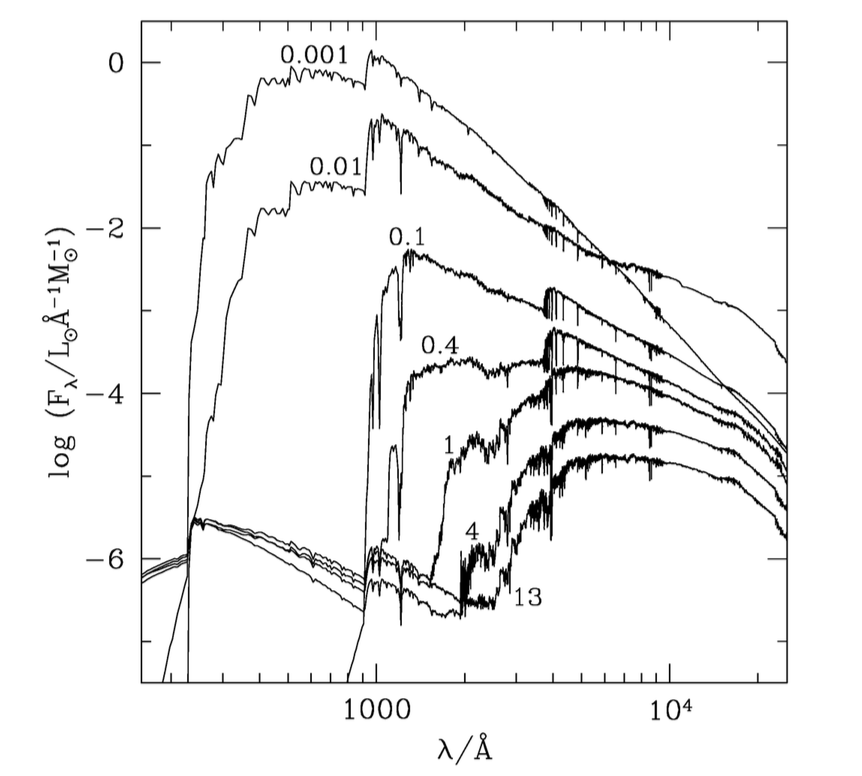
\includegraphics[width=0.6\textwidth]{bc03_spectra.png}
\caption{\footnotesize{\emph{Spectral evolution of an SSP at solar metallicity}}}
\label{fig:BC03_spectra}
\end{figure} 


\subsubsection{Interpretation of Galaxy Spectra}
Using data from the EDR of SDDS, to interpret these spectra the authors use the MOPED data compression algorithm \citep{Heavens2000}. Several advantages to using this approach described throughout the paper. The model can be used to reliably to measure the contamination of Balmer emission lines by underlying stellar absoprtion in galaxies. Can't really be bothered reading the rest of this paper, need to sort out the sky situation first.   



%%%%%%%%%%%%%%%%%%%%%%%%%%%%%%%%%%%%%%%%%%%%%%%%%%%%%%%%%%%%%%%%%%%%%%%%%%%%%%%%%%%%%%%%%%%%%%%%%%%%%%%%%




\section{Steidel: Strong Nebular line ratios in the spectra of redshift 2-3 galaxies. KBSS MOSFIRE}
\subsection{Abstract and Introduction}
First results from a deep NIR spectroscopic survey covering the 15 fields of the Keck Baryonic Structure Survey using MOSFIRE on the Keck 1 telescope. The locus of $z\sim 2.3$ galaxies in the BPT diagnostic diagram exhibits a disjoint but similarly tight relationship between the ratios NII/Ha and OIII/Hb as compared to local galaxies. Using photoionisation models the author argues that the offset at this redshift with respect to locally is due to a harder ionising radiation field, higher ionisation parameter and higher N/O at a given O/H than applies to most local galaxies. Despite much effort \citep{Mannucci2010}, \citep{ForsterSchreiber2009}, \citep{Cullen2014}, \citep{Troncoso_2014}, \citep{Wuyts_2014}, \citep{Henry2013}, \citep{Maiolino2008} samples of high redshift galaxies for which a reasonably complete set of strong lines has been measured remain very small. The advent of NIR spectrographs on 8-10m telescopes has long promised to revolutionise nebular spectroscopy of high redshift galaxies, by vastly enlarging the sample sizes and making very deep spectroscopy observationally practical. Strong lines tell us about density, OII3727,3729 and SII 6718,6732,  temperature OIII4960,5008/OII4364, ionisation state OIII4969,5008/OII3727,3729 and metallicity (mainly $R_{23}$ and NII6585/Ha) by taking different combinations of their ratios. Additionally the BPT diagnostic is used to determine what the dominant ionisation mechanism within a galaxy is, providing a relatively clean way to distinguish between nebular emisison which has been ionised by AGN activity and by the UV radiation field. Paper seeking to discover whether since the BPT diagram is shifted, does that mean applying locally calibrated emission line ratios to the high-z universe may be more complicated than hoped? \\ 
Large differences in the calibrations of oxygen abundance indicators mainly from whether they were calibrated theoretically or by using sensitive measurements of the electron temperature, the so called `direct $T_{e}$' method. The direct method tends to provide more accurate results, but it requires measurement of the weak emission lines which are unobservable at high metallicity and high redshift, where they are shifted into regions of the spectrum plagued by higher levels of terrestial background. It has been shown that it is possible to force the different strong line calibration techniques to agree within 0.03 dex in the local universe \citep{Kewley_2008}, however these give only relative abundances. Also the heart of this paper is answering whether this can be applied to the high-z universe, clearly very desirable, and to answer this we must know if the physics of high-z nebular regions are different to those at $z=0$. Why is NIR spectroscopy so hard? From the ground there are large gaps in the atmospheric transmission and beyond a few microns there is substantial background. How can you tell if the gas-phase metallicity is evolving of whether there has been a change on the dependence of measured line intensity and metallicity? \\ 

\subsection{Observations and Data}
Real time observations, mask re-assignment based on a set of priority flags. Sounds like really cool stuff, all trying to maximise the scientific return from the telescope. 





%%%%%%%%%%%%%%%%%%%%%%%%%%%%%%%%%%%%%%%%%%%%%%%%%%%%%%%%%%%%%%%%%%%%%%%%%%%%%%%%%%%%%%%%%%%%%%%%%%%%%%%%%%

\section{Distance Measures in Cosmology}\label{sec:cosmology_distance}
\subsection{Cosmographic Parameters}
Relevant to distance in the parameter $D_{H}$ which is known as the hubble distance, given simply by the speed of light multiplied by the hubble time (inverse hubble constant). The other cosmological parameters, $\Omega_{M}, \Omega_{\Lambda} and \Omega_{k}$ determine the mass density of the universe and hence the time evolution of the metric and the cosmological distance to points at certain redshift.
\subsection{Redshift}\label{subs:redshift}
The redshift of an object is the fractional doppler shift in its spectral lines caused by radial motion. Redshift is directly observable and radial velocity is not; these notes concentrate on observables. There is a difference between the observed redshift and cosmological redshift of an object, caused by the peculiar motion of that object. Cosmological redshift is taken to mean the part of the redshift which is due purely to the expansion of the universe. The redshift values used from here on out will solely relate to this cosmological redshift, which is a far more useful quantity. The two values are related using the relation: 
\begin{equation}
v_{pec} = \frac c{z_{obs} - z_{cos}}{(1 + z)}	
\end{equation}
For small distances the different measures $D_{L}, D_{A}$ etc converge and the simple Hubble approximation can be used: $v_{rec} = H_{0}D$. However this is only true for the very local universe and is not true in general. Generally, the redshift of an object is related to the scale factor via $1 + z = \frac{a(t_{o})}{a(t_{e})}$ where $a(t_{o})$ is the size of the universe at the time the light was observed.
\subsection{Comoving Distance}\label{subs:comoving_distance}
A small comoving distance between two nearby objects in the universe is the distance between them which remains constant with epoch if the two objects are moving together with the Hubble flow. The total comoving distance to an object at redshift z is given by integrating these infinitesimal constributions from objects close to each other, i.e. by the equation in section \ref{meeting_2}. The line-of-sight comoving distance between two nearby events (ie, close in redshift or distance) is the distance which we would measure locally between the events today if those two points were locked into the Hubble flow. It is also in many ways the fundamental distance measure, as all other measures are derived quite simply in terms of this. 
\subsection{Transverse Comoving Distance}\label{subs:transverse_comoving_distance}
This is denoted by $D_{M}$ and is related to the comoving distance by the formulae presented in the Hogg paper. The two quantities are analogous in a flat universe, but when spatial curvature in introduced there is either a sin or sinh function. 
\subsection{Angular Diameter Distance}\label{subs:Angular Diameter distance}
The angular diameter distance DA is defined as the ratio of an object’s physical transverse size to its angular size (in radians). This distance measure doesn't increase indefinitely and turns over at $z \sim 1$, where objects of fixed physical size at higher redshift than this appear larger.
\subsection{Luminosity Distance}\label{subs:Luminosity distance}
The luminosity distance $D_{L}$ is defined by the relationship between bolometric (ie, integrated over all frequencies) flux S and bolometric luminosity L:
\begin{equation}
	D_{l} = \sqrt \frac{L}{4\pi S}
\end{equation}
And after some calculation it can be shown that this is related to the transverse comoving distance, which will be computed first by the numerical integral, by $D_{L} = (1 + z)D_{M}$. If the concern is not with bolometric quantities but rather with differential flux $S_{\nu}$ and luminosity $L_{\nu}$ , as is usually the case in astronomy, then a correction, the k-correction, must be applied to the flux or luminosity because the redshifted object is emitting flux in a different band than that in which you are observing. The remainder of this section then describes in detail the definition of the k-correction.

\subsection{Comoving Volume}\label{subs:Comoving Volume}
The comoving volume $V_{C}$ is the volume measure in which number densities of non-evolving objects locked into Hubble flow are constant with redshift.

\subsection{Lookback time and age}\label{subs:lookback time}
Hello

%%%%%%%%%%%%%%%%%%%%%%%%%%%%%%%%%%%%%%%%%%%%%%%%%%%%%%%%%%%%%%%%%%%%%%%%%%%%%%%%%%%%%%%%%%%%%%%%%%%%%%%%%%%%%%%%


\section{Brinchmann Physical Properties}\label{sec:Brinchmann_properties}
\subsection{Introduction}
Based on the results of previous studies, a picture has emerged whereby more massive galaxies undergo a larger fraction of their star formation at early times than less massive ones. This has often been said to present a challenge to existing models of galaxy formation. Initial studies with relatively small galaxy samples, but with the advent of large fibre-fed surveys it is now possible to dramatically increase the size of the galaxy sample. This work is aimed at probing the SFH history of the universe as a whole, as there are wide discrepancies between the evolution of the SFR above $z = 3$. One of the key questions is what physical parameters drive the changes in the SFR in individual galaxies. It is therefore of crucial importance to investigate empirically what global quantities correlate strongly with star formation activity. Fitting all strong emission lines simultaneously. 



%%%%%%%%%%%%%%%%%%%%%%%%%%%%%%%%%%%%%%%%%%%%%%%%%%%%%%%%%%%%%%%%%%%%%%%%%%%%%%%%%%%%%%%%%%%%%%%%%%%%%%%%%%%%%%%%%

\review
\label{background-review}

\progress
\label{progress}

\summary
\label{summary}

%%%%%%%%%%%%%%%%%%%%%%%%%%%%%%%%%%%%%%%%%%%%%%%%%%%%%%%%%%%%%%%%%%%%%%%%%%%%%%%%%%%%%%%%%%%%%%%%%%%%%%%%%%%%%%%%%%

\section{Definitions}
\begin{itemize}
\item \underline{Dynamic Range}: The ratio of the largest to the smallest possible values of a changeable quantity.
\item \underline{Synthesis}: The combination of components or elements to combine a collective whole. e.g. the evolutionary synthesis of a population of stars.
\item \underline{efficacy}: The ability to produce the desired or intended result
\item \underline{calorimetric measure}: Young stellar population transferring heat to the dust particles, which will emit at a certain peak wavelength
\item \underline{bolometric luminosity}: The luminosity of an object after taking into account all frequencies of electromagnetic waves and extinction and absorption in the Earth's atmosphere.
\item \underline{coeval}: Having the same age or date of origin
\item \underline{Interloper}: Becoming involved in a situation where it is considered not to belong	
\item \underline{abscissas}: In the context of mathematics, the abscissa is the perpendicular distance of a point from the y-axis. The distance parallel to the y-axis is called the ordinate
\item \underline{Gaseous Nebulae}: Gaseous nebulae are optically visible clouds of gas present in our Galaxy and in other galaxies
\item \underline{Forbidden Line}: Emission lines observed in the astronomical spectra of gaseous nebulae, but not from the spectra of the same elements in a laboratory on Earth. The term forbidden is misleading, more appropriate would be highly unlikely. The gas cannot be sufficiently rarefied on Earth, and instead of transitioning from a higher energy level to a lower one via photo-emission, the electrons are many orders of magnitude more likely to do so via collisional de-excitation either with another electron or with the walls of a container.
\item \underline{Lyman alpha Forest}: Observed in the spectra of bright distant objects. The Lyman alpha photons emitted by the object are absorbed by clouds of intergalactic neutral hydrogen between us and the object. Each absorption, at different degrees of redshift leaves its fingerprint in the spectrum. Used to diagnose the frequency and density of clouds of intergalactic neutral hydrogen
\item \underline{Lyman Break Galaxy}: Galaxies observed in at least one filter shortwards and longwards of the Lyman limit show this break in their emission. Colour selection technique whereby high redshift galaxies, or galaxies at a particular redshift, can be picked out. This feature is present in star forming galaxies, where light shortwards of the Lyman limit is almost completely absorbed by dust and nebular emission clouds around star forming regions - so the galaxy exhibits a `break' in its SED at the shifted location of the 91.2nm Lyman limit.
\item \underline{Auroral Line}: Emission between the second lowest and lowest excited states 
\item \underline{Nebular Line}: Emission between the first excited and ground states. The ratio of the auroral and nebular emission lines is extremely sensitive to electron temperature and is the preferred method of estimating metal abundances in HII regions. However the auroral line becomes very weak at metallicites above 0.5 solar, and so it difficult to measure in practice. As a result people resort to calibrated ratios of strong, forbidden emission lines.  
\end{itemize}



%%%%%%%%%%%%%%%%%%%%%%%%%%%%%%%%%%%%%%%%%%%%%%%%%%%%%%%%%%%%%%%%%%%%%%%%%%%%%%%%%%%%%%%%%%%%%%%%%%%%%%%%%%%%%%


\section{General Interest and Quotes}

The cameras on Hubble and MER do not take color pictures, however. Color images from both spacecraft are assembled from separate black and white images taken through color filters. For one image, the spacecraft have to take three pictures, usually through a red, a green, and a blue filter and then each of those photos gets downlinked to Earth. They are then combined with software into a color image. This happens automatically inside off-the-shelf color cameras that we use here on Earth. But the MER Pancams have 8 different color filters while Hubble has almost 40, ranging from ultraviolet `bluer' than our eyes can see through the visible spectrum, to infrared `redder' than what is visible to humans. This gives the imaging teams infinitely more flexibility and sometimes, artistic license. Depending on which filters are used, the color can be closer or farther from `reality'. \\
In the case of the Hubble, Levay explained, the images are further adjusted to boost contrast and tweak colors and brightness to emphasize certain features of the image or to make a more pleasing picture. \\ 
Hubble can also produce color-calibrated images. Its `UniverseDial' would be standard stars and lamps within the cameras whose brightness and color are known very accurately. However, Hubble’s mission is not to produce images that faithfully reproduce colors. `For one thing that is somewhat meaningless in the case of most of the images,' said Levay, since we generally couldn’t see these objects anyway because they are so faint, and our eyes react differently to colors of very faint light. But the most important goal of Hubble is produce images that convey as much scientific information as possible.

%%%%%%%%%%%%%%%%%%%%%%%%%%%%%%%%%%%%%%%%%%%%%%%%%%%%%%%%%%%%%%%%%%%%%%%%%%%%%%%%%%%%%%%%%%%%%%%%%%%%%%%%%%%%%%%%%%

\section{Questions}
\subsection{SFR diagnostics}
\begin{itemize}
\item Is there a reason why initially it would be assumed that high redshift galaxies would not be star forming? 
\item What does it mean a gradual change in the stellar absorption spectrum, from K-giant dominated to A star dominated? 
\item Page 193: `A grid of Stellar evolution tracks...' what does that mean? Also `Converted into broadband luminosities (or spectra) using stellar atmosphere models or spectral libraries' what does that mean? 
\item The article refers to sythesis models in the context of single age populations. What is the approach for populations of stars which are not single age? 
\item Why do the evolutionary synthesis models give relations between the sSFR and the integrated colour of the galaxy? Why choose the integrated colour as the x-axis of the plot? 
\item Confirming the meaning of the use of dex. e.g. differing over a full range of $\sim 0.3$dex.
\item The best determinations of the extinction are based on two component radidative transfer models...
\item The meaning of `Nebular' emission lines, and how are they re-emitting the light which is `shortward' of the Lyman limit. And only young massive stars are emitting these lines? What is the connection with a flux of ionising photons? 
\item Importance of the escape fraction of ionising photons for the measurement of SFR from nebular emission lines.
\item The SFR vs $L_{FIR}$ conversion is derived using synthesis models as described above. Linking with the above questions surrounding these synthesis models. Then directly leading on from this quote on page 201: `In the optically thick limit it is only necessary to model the bolometric luminosity of the stellar population'
\item

\end{itemize}



%%%%%%%%%%%%%%%%%%%%%%%%%%%%%%%%%%%%%%%%%%%%%%%%%%%%%%%%%%%%%%%%%%%%%%%%%%%%%%%%%%%%%%%%%%%%%%%%%%%%%%%%%%%%%%%%%%%%%%%%



\subsection{Metallicity Measurement}\label{que:metallicity}
\begin{itemize}
\item Line ratios being used to measure metallicity - which ratio is the best? 
\item Accurate abundance measurements require the determination of the electron 
\item What causes the sky background to be so much higher in the NIR than in the optical?
\item The stellar metallicity vs. the gas metallicity. Which is used more as a tracer of galaxy metallicity and which is easier to measure? 
\item What is constituting the continuum emission observed from emission nebulae? Combination of the HI Paschen and Balmer continua and a reflective continuum from starlight scattered by dust.
\item Two dimensional spectral analysis. Beyond the scope of the Maiolino paper.
\item The emission coefficient j
\item The careful avoidance of galaxies hosting an AGN. AGN contribute to the ionising flux of photons and so alter the ratio of emission lines. In this case the metallicity diagnostic diagrams calibrating on star forming galaxies are not usable. How then is the metallicity measured for galaxies hosting AGN? What fraction of galaxies host an AGN? 
\item The lower and the upper branch of the $R_{23}$ ratio - how does the method yield two different metallicity estimates?
\item Quoting the Oxygen abundance in terms of $12 + log\frac{O}{H}$? Why? Where does this come from? 
\end{itemize}

\subsection{Cosmology calculator}\label{que:cosmology_calc}
\begin{itemize}
	\item When computing the angular diameter distance do I also need to code in the cases for a non-flat universe?
	\item What level of precision are we looking for with the different distance measures?
	\item When I use the cosmology calculator with $\Omega _{\Lambda}$ bigger than 1.5 it gives nonsensical answers. Why? 
	\item How to be sure which step size to use when computing these integrals?
	\item Convergence after successive calls to the initial Trapezoidal integral? 
	\item Romberg integration??
	\item Integrating along a given axis?
\end{itemize}

\subsection{Data Analysis}\label{que:data_analysis}
\begin{itemize}
	\item What does simultaneously fitting the emission lines mean? De-blending happens automatically
	\item Where can I find out more about these spectra? i.e. flux units etc 
	\item Why are there so many data units associated with each fits file extracted?
	\item Some of the values show negative flux, how is that possible?
	\item Masking the emission line spikes 
	\item What precision are we wanting here? The task of fitting all of these emission lines is pretty much the subject of an entire SDSS paper and is totally non-trivial
	\item Why are the SFRs described in the galSpecextra table of SDSS reported in terms of PDFs? 
	\item Going through step by step what is the best way to analyse these spectra
	\item Having trouble interpreting the formula in the Kennicutt review for the SFR calibration
	\item SDSS Vacuum corrected wavelengths - only get good fit using these
	\item Difference between compound model which fits the gaussians simultaneously and individual models which fit the gaussians one by one for each of the emission lines? 
	\item Is the error on the flux sigma or is it the FWHM? 
	\item Where should the for loop over the file names be? At the end or within the methods? 
	\item How to compute the equivalent width properly? 
	\item Should the model also include a coefficient to vary the height of the gaussian? i.e. also accounting for absorption?
	\item When the emission spectra are modelled does this also include the emission lines or is it just the continuum emission from the galaxy being synthesised?
	\item When plotting the cross correlation function, how many shifts along the redshift axis should I have? As many as possible? Probably don't want anything more than a second significant figure in the redshift at the moment.	
	\item Are the weak emission lines of high redshift galaxies a result of them being early type, or a result of us being much further away and so the S/N is poorer? 
	\item Cross correlation function - is this for each individual emission line or do I average over all of the flux multiplications?
	\item Why are we doing this SED cross correlation function when we have the galaxy spectrum? Surely it is obvious what the redshift is from the shift of H-alpha?
	\item Constructing the composite spectra?
	\item How to use a weights vector when have error bars on both the x and y axes? 
	\item Starburst99 the two empirical stellar libraries available in the code - one for the milky way and one for the MC. What does this mean? What is a stellar library?
	\item Computing metallicity from the likelihood distribution - Bayesian approach. Specifically in the Tremonti et al. SDSS paper.
	\item What do the colours mean in astronomical images? If recorded with a CCD, surely the voltage is just telling us about the liberated number of electrons, how then do we see all of these pretty colours in cameras and telescope images? Calibration. Each pixel has a wavelength associated with it, and so we know what colour is associated with that as well? Works in the optical, but when we're looking at IR pictures, why are they always represented by red? Surely we don't know what these would look like? 
	\item What are the advantages of KMOS over SINFONI, also a VLT near IR spectrograph?
	\item Construction of a composite spectrum - both wavelength binning and redshifting of the different constituent spectra necessary?
	\item 

\end{itemize}

\subsection{Analysis Pipeline}\label{que:analysis_pipeline}
\begin{itemize}
	\item The manual which is 184 pages long - is this important for me to read at some stage?
\end{itemize}

%%%%%%%%%%%%%%%%%%%%%%%%%%%%%%%%%%%%%%%%%%%%%%%%%%%%%%%%%%%%%%%%%%%%%%%%%%%%%%%%%%%%%%%%%%%%%%%%%%%%%%%%%%%%%%%%%%%%%%%%

\clearpage 
\bibliographystyle{apj.bst}
%\bibliography{/usr/local/texlive/texmf-local/bibtex/bib/ojt.bib}
\bibliography{/Users/owenturner/Documents/PhD/KMOS/Latex/Literature_Review/Bibtex/library.bib}

\end{document}
